\setcounter{ex}{0}
\section*{TỔNG HỢP VDC - CHƯƠNG I}
\Opensolutionfile{ans}[ans/ansBTchoice]
\TN
\begin{ex}%[2D1C5-7]
Tìm được trên đồ thị $(C)$ của hàm số $y=\dfrac{x^2+4x+5}{x+2}$ hai điểm $M(a;b)$ và $N(c;d)$ có khoảng cách đến đường thẳng $\Delta\colon 3x+y+6=0$ nhỏ nhất. Khi đó $a+b+c+d$ bằng
\choice
{$4$}
{$9$}
{$-9$}
{\True $-4$}
\loigiai
{Tập xác định $\mathscr{D}=\mathbb{R}\setminus\{-2\}$.
Gọi $M\left(x_0;y_0\right) \in (C)$. Ta có $x_0\neq -2$ và $y_0=\dfrac{x_0^2+4x_0+5}{x_0+2}$.\\
Khoảng cách từ $M$ đến đường thẳng $\Delta\colon 3x+y+6=0$ là
$$\mathrm{d}\left(M,\Delta\right)=\dfrac{1}{\sqrt{10}}\left|\dfrac{4x_0^2+16x_0+17}{x_0+2}\right|=\dfrac{1}{\sqrt{10}}\left|4\left(x_0+2\right)+\dfrac{1}{x_0+2}\right|.$$
Hàm số $f(t)=4t+\dfrac{1}{t}$ với $t\neq 0$ có $f'(t)=\dfrac{4t^2-1}{t^2}$ và $f'(t)=0\Leftrightarrow 4t^2-1=0\Leftrightarrow t=\pm \dfrac{1}{2}$.\\
Bảng biến thiên \begin{center}

\begin{tikzpicture}
\tkzTabInit[nocadre=false, lgt=1.2, espcl=2.5, deltacl=0.6]{$t$/1.2,$f'(t)$/0.6,$f(t)$/2}
{$-\infty$, $-\dfrac{1}{2}$, $0$, $\dfrac{1}{2}$, $+\infty$}
\tkzTabLine {,+,0,-,d,-,0,+,}
\tkzTabVar{-/$-\infty$, +/$-4$, -D+/$-\infty$/$+\infty$,-/$4$, +/$+\infty$}
\end{tikzpicture}
\end{center}
Suy ra $\min\limits_{t\neq 0} \left|f(t)\right|=4$ khi $t=\pm\dfrac{1}{2}$.\\
Do đó $\min\mathrm{d}(M,\Delta)=\dfrac{4}{\sqrt{10}}$ khi
$x_0+2=\pm\dfrac{1}{2} \Leftrightarrow \hoac{& x_0=-\dfrac{3}{2} \Rightarrow y_0=\dfrac{5}{2}\\ &x_0=-\dfrac{5}{2} \Rightarrow y_0=-\dfrac{5}{2}.}$\\
Như thế có hai điểm thoả yêu cầu bài toán là $M\left(-\dfrac{3}{2};\dfrac{5}{2}\right)$ và $N\left(-\dfrac{5}{2};-\dfrac{5}{2}\right)$.\\
Vậy $a+b+c+d=-\dfrac{3}{2}+\dfrac{5}{2}-\dfrac{5}{2}-\dfrac{5}{2}=-4$.
}
\end{ex}

\begin{ex}%[Dự Án Giảng 12 4 in 1, Lê Văn Toàn]%[2D1C5-6]
Trên đồ thị của hàm số $y=\dfrac{3x}{x-2}$ có điểm $M\left(x_0;y_0\right)$ $\left( \text{ với }x_0<0\right)$ sao cho tiếp tuyến tại điểm đó cùng với các trục tọa độ tạo thành một tam giác có diện tích bằng $\dfrac{3}{4}$. Khi đó $x_0+2y_0$ bằng
\choice
{$\dfrac{1}{2}$}
{$-1$}
{$-\dfrac{1}{2}$}
{\True $1$}
\loigiai{
Gọi $(C)$ là đồ thị của hàm số $y=\dfrac{3x}{x-2}$, $M\left(x_0;y_0\right)\in (C)$, suy ra $y_0=\dfrac{3x_0}{x_0-2}$ và $y'\left(x_0\right)=\dfrac{-6}{\left(x_0-2\right)^2}$.\\
Phương trình tiếp tuyến của $(C)$ tại $M\left(x_0;y_0\right)$ là $\Delta\colon y=\dfrac{-6}{\left(x_0-2\right)^2}\left(x-x_0\right)+\dfrac{3x_0}{x_0-2}$.\\
Gọi $A=\Delta \cap Ox\Rightarrow -6x+3x^2_0=0\Rightarrow x=\dfrac{x^2_0}{2}\Rightarrow A\left(\dfrac{x^2_0}{2};0\right)$.\\
Gọi $B=\Delta\cap Oy\Rightarrow y=\dfrac{6x_0}{\left(x_0-2\right)^2}+\dfrac{3x_0}{x_0-2}=\dfrac{3x_0^2}{\left(x_0-2\right)^2}\Rightarrow B\left(0;\dfrac{3x_0^2}{\left(x_0-2\right)^2}\right).$\\
Ta có $$S_{OAB}=\dfrac{1}{2}OA\cdot OB=\dfrac{1}{2}\cdot \dfrac{x^2_0}{2}\cdot \dfrac{3x^2_0}{\left(x_0-2\right)^2}=\dfrac{3}{4}\Leftrightarrow x^4_0=\left(x_0-2\right)^2\Leftrightarrow \hoac{&x^2_0=x_0-2\\&x^2_0=-x_0+2}\Leftrightarrow \hoac{&x_0=1\\&x_0=2.}$$
Do $x_0<0$ nên  nhận $x_0=-2\Rightarrow y_0=\dfrac{3}{2}$.\\
Vậy $x_0+2y_0=1$.
}
\end{ex}

\begin{ex}%[Mức độ C]%[2D1C5-3]
Tìm tất cả các giá trị thực của $m$ để phương trình $|x^4-2x^2-3|=2m-1$ có đúng $6$ nghiệm thực phân biệt.
\choice{$1<m<\dfrac{1}{3}$}{$4<m<5$}{$3<m<4$}{\True $2<m<\dfrac{5}{2}$}
\loigiai{Xét $g(x)=x^4-2x^2-3$; $g'(x)=4x^3-4x$.\\
$g'(x)=0\Leftrightarrow 4x^3-4x=0 \Leftrightarrow \left[\begin{array}{l}
x=0\\x=1\\x=-1.
\end{array}\right.$ \\
Bảng biến thiên của hàm số $g(x)$
\begin{center}

\begin{tikzpicture}
\tkzTabInit[nocadre=false, lgt=1.5,espcl=3.5]
{$x$/1,$g'(x)$/1,$g(x)$/2}
{$-\infty$,$-1$,$0$,$1$,$+\infty$}
\tkzTabLine{,-,0,+,0,-,0,+, }
\tkzTabVar{+/$+\infty$,-/$-4$,+/$-3$,-/$-4$,+/$+\infty$/}
\end{tikzpicture}
\end{center}
Bảng biến thiên của hàm số $f(x)=|x^4-2x^2-3|$ là
\begin{center}

\begin{tikzpicture}[scale=0.75]
\tkzTabInit[nocadre=false, lgt=1.5,espcl=3.5]
{$x$/1,$f(x)$/2}
{$-\infty$,$-\sqrt{3}$,$-1$,$0$,$1$,$\sqrt{3}$,$+\infty$}
\tkzTabVar{+/$+\infty$,-/$0$,+/$4$,-/$3$,+/$4$,-/$0$,+/$+\infty$/}
\end{tikzpicture}
\end{center}
Để phương trình $|x^4-2x^2-3|=2m-1$ có đúng $6$ nghiệm thực phân biệt khi và chỉ khi $$ 3<2m-1<4 \Leftrightarrow 2<m<\dfrac{5}{2}.$$.
}
\end{ex}

\begin{ex}%[Mức độ C]%[2D1C5-3]
Cho hàm số $y=f(x)$ liên tục trên $\mathbb{R}$ và có đồ thị như hình vẽ dưới đây. Tập hợp tất cả các giá trị thực của tham số $m$ để phương trình $f(x^2+2x-2)=3m+1$ có nghiệm thuộc khoảng $[0;1]$.
\begin{center}
\begin{tikzpicture}[>=stealth]
\draw [->] (-3.5,0)--(1.5,0);
\draw [->] (0,-1)--(0,5);
\draw (0,0) node[below right]{$O$};
\draw (1.5,0) node[below]{$x$};
\draw (0,5) node[below left]{$y$};
\draw (1,0) node[below]{$1$};
\draw (0,4) node[below left]{$4$};
\draw (-2,0) node[below]{$-2$};
\clip (-4,-1) rectangle (5,5);
\draw [thick,samples=100] plot[domain=-5:5](\x,{(\x)^3+3*(\x)^2});
\draw[dashed] (0,4) -- (1,4) --(1,0);
\fill[black] (1,4) circle(2pt);
\fill[black] (-2,4) circle(2pt);
\fill[black] (0,0) circle(2pt);
\draw[dashed] (0,4) -- (-2,4) --(-2,0);
\draw (1.1,5) node[below right]{$f(x)$};
\end{tikzpicture}
\end{center}
\choice
{$[0;4]$}
{$[-1;0]$}
{$[0;1]$}
{\True $\bigg[-\dfrac{1}{3};1\bigg]$}
\loigiai{Đặt $t=x^2+2x-2$, Với $x \in [0;1] \Rightarrow t \in [-2;1].$\\
Để phương trình $f(x^2+2x-2)=3m+1$ có nghiệm thuộc đoạn $[0;1]$ khi và chỉ khi phương trình $f(t)=3m+1$ có nghiệm thuộc $[-2;1].$\\ Do đó $ 0\leq m \leq 4 \Leftrightarrow -\dfrac{1}{3}\leq m \leq 1$.\\
Vậy $m \in \bigg[-\dfrac{1}{3};1\bigg]$}
\end{ex}

\begin{ex}%[Dự án TL12New-4in1-NCT]%[2D1C4-2]
Tìm tất cả các giá trị thực của tham số $m$ sao cho đồ thị hàm số $y=\dfrac{x+2}{\sqrt{mx^2+1}+\sqrt{(1-m)x^2+1}}$ có hai tiệm cận ngang.
\choice
{$m>0$}
{$m<1$}
{\True $0\leq m\leq 1$}
{$0<m<1$}
\loigiai{
Xét các trường hợp
\begin{itemize}
\item $m<0$ hoặc $m>1$, khi đó $\lim\limits_{x\to \infty}y$ không tồn tại nên đồ thị hàm số không thể có hai tiệm cận ngang.
\item Với $m=0$ hoặc $m=1$ thì hàm số trở thành $y=\dfrac{x+2}{1+\sqrt{x^2+1}}$. Đồ thị hàm số có đúng hai đường tiệm cận ngang $y=1$ và $y=-1$. Do đó $m=0$ và $m=1$ thỏa mãn yêu cầu bài toán.
\item Với $0<m<1$ ta có:
\begin{enumerate}[*]
\item $\lim\limits_{x\to +\infty}y=\lim\limits_{x\to +\infty}\dfrac{1+\dfrac{2}{x}}{\sqrt{m+\dfrac{1}{x^2}}+\sqrt{1-m+\dfrac{1}{x^2}}}=\dfrac{1}{\sqrt{m}+\sqrt{1-m}}$
\item $\lim\limits_{x\to -\infty}y=\lim\limits_{x\to -\infty}\dfrac{1+\dfrac{2}{x}}{-\sqrt{m+\dfrac{1}{x^2}}-\sqrt{1-m+\dfrac{1}{x^2}}}=\dfrac{-1}{\sqrt{m}+\sqrt{1-m}}$.
\end{enumerate}
Do đó đồ thị có hai tiệm cận ngang khi và chỉ khi\\ $\dfrac{1}{\sqrt{m}+\sqrt{1-m}}\neq \dfrac{-1}{\sqrt{m}+\sqrt{1-m}} \Leftrightarrow \dfrac{1}{\sqrt{m}+\sqrt{1-m}}\neq 0$ (hiển nhiên).
\end{itemize}
Tóm lại, $0\leq m\leq 1$ là các giá trị của $m$ thỏa mãn yêu cầu bài toán.
}
\end{ex}

\begin{ex}%[BG-12NEW-4in1, Nguyen Huynh]%[2D1C4-1]
Đồ thị hàm số $y=\log\dfrac{x^2-4x-5}{x^2-4}$ có tất cả bao nhiêu đường tiệm cận?
\choice
{$1$}
{$3$}
{\True $5$}
{$2$}
\loigiai{
Tập xác định của hàm số $\mathscr{D}=(-\infty;-2)\cup(-1;2)\cup(5;+\infty)$.\\
Mà $\lim\limits_{x\to \pm\infty}\log\dfrac{x^2-4x-5}{x^2-4}=\log 1=0$, suy ra $y=0$ là tiệm cận ngang của đồ thị hàm số.\\
Mà $\lim\limits_{x\to -2^-}\log\dfrac{x^2-4x-5}{x^2-4}=\lim\limits_{x\to +\infty}\log (x)=+\infty$, suy ra $x=-2$ là tiệm cận đứng của đồ thị hàm số.\\
Mà $\lim\limits_{x\to 2^-}\log\dfrac{x^2-4x-5}{x^2-4}=\lim\limits_{x\to +\infty}\log (x)=+\infty$, suy ra $x=2$ là tiệm cận đứng của đồ thị hàm số.\\
Mà $\lim\limits_{x\to -1^+}\log\dfrac{x^2-4x-5}{x^2-4}=\lim\limits_{x\to 0^+}\log (x)=-\infty$, suy ra $x=-1$ là tiệm cận đứng của đồ thị hàm số.\\
Mà $\lim\limits_{x\to 5^+}\log\dfrac{x^2-4x-5}{x^2-4}=\lim\limits_{x\to 0^+}\log (x)=-\infty$, suy ra $x=5$ là tiệm cận đứng của đồ thị hàm số.\\
Vậy đồ thị hàm số có $5$ đường tiệm cận.
}
\end{ex}

\begin{ex}%[THPTGQ 2018, mã 103, MĐ4]%[2D1C2-6]
Có bao nhiêu giá trị nguyên của tham số $m$ để hàm số $y=x^8+(m-4)x^5-(m^2-16)x^4+1$ đạt cực tiểu tại $x=0$.
\choice
{\True $8$}
{Vô số}
{$7$}
{$9$}
\loigiai{
Ta có $y'=8x^7+5(m-4)x^4-4(m^2-16)x^3$. \\
Đặt $g(x)=8x^4+5(m-4)x-4(m^2-16)$. Có $2$ trường hợp cần xét liên quan $(m^2-16)$:
\begin{itemize}
\item Trường hợp 1: $m^2-16=0 \Leftrightarrow m=\pm 4$.
\begin{itemize}
\item[+] Khi $m=4$ ta có $y'=8x^7 \Rightarrow x=0$ là điểm cực tiểu.
\item[+] Khi $m=-4$ ta có $y'=x^4(8x^4-40) \Rightarrow x=0$ không là điểm cực tiểu.
\end{itemize}
\item Trường hợp 2: $m^2-16\ne 0 \Leftrightarrow m\ne \pm 4$. Khi đó $x=0$ không là nghiệm của $g(x)$.\\
Ta có $x^3$ đổi dấu từ $-$ sang $+$ khi qua $x_0=0$, do đó\\
$y'=x^3\cdot g(x)$ đổi dấu từ $-$ sang $+$ khi qua $x_0=0 \Leftrightarrow \lim\limits_{x \to 0} g(x)>0 \Leftrightarrow m^2-16<0$.
\end{itemize}
Kết hợp các trường hợp giải được ta nhận $m \in \{-3;-2;-1;0;1;2;3;4\}$.}
\end{ex}

\begin{ex}%[THPTGQ 2018, mã 102, MĐ4]%[2D1C2-6]
Có bao nhiêu giá trị nguyên của tham số $m$ để hàm số
\begin{eqnarray*}
y =x^8+ (m - 1)x^5- (m^2- 1)x^4+ 1
\end{eqnarray*}
đạt cực tiểu tại $x = 0$?
\choice
{$3$}
{\True $2$}
{Vô số}
{$1$}
\loigiai{
Ta có $ y'=8x^7+5(m-1)x^4-4(m^2-1)x^3+1=x^3\left[ 8x^4+5(m-1)x-4(m^2-1) \right]  $,
$$ y'=0\Leftrightarrow \hoac{&x=0\\&8x^4+5(m-1)x-4(m^2-1)=0.\ \ (*)} $$
\begin{itemize}
\item Nếu $ m=1 $ thì $ y'=8x^7 $, suy ra hàm số đạt cực tiểu tại $ x=0 $.
\item Nếu $ m=-1 $ thì $ $$y'=0\Leftrightarrow\hoac{&x=0\\&8x^4-10x=0}\Leftrightarrow\hoac{&x=0\mbox{ (nghiệm kép)}\\&x=\sqrt[3]{\dfrac{5}{4}.}}$
Do đó $x=0$ không phải là điểm cực trị.
\item Nếu $ m\ne\pm1 $ thì $ x=0 $ là nghiệm đơn.\\
Đặt $ g(x)=8x^4+5(m-1)x-4(m^2-1) $. Hàm số đã cho đạt cực tiểu tại $ x=0 $ khi chỉ khi $$ \lim_{x\to 0^{-}}g(x)>0\Leftrightarrow -4(m^2-1)>0\Leftrightarrow m^2-1<0\Leftrightarrow -1<m<1. $$
Vì $ m\in\mathbb{Z} $ nên $ m=0 $.
\end{itemize}
Vậy giá trị $ m $ thỏa mãn yêu cầu bài toán là $ m=0 $, $ m=1 $.
}
\end{ex}

\begin{ex}%[MĐ4]%[2D1C2-6]
Có bao nhiêu giá trị nguyên dương của tham số $ m $ không vượt quá $ 2019 $ để hàm số $ f(x) = \dfrac{x^2}{8} + \sqrt{x + m + 2} $ không có điểm cực trị?
\choice
{ $ 0 $}
{\True$ 1 $}
{$ 2018 $}
{$ 2019 $}
\loigiai{
Tập xác định  $ \mathscr{D} = [ - m - 2;+ \infty)$.\\
Ta thấy \allowdisplaybreaks{
\begin{eqnarray*}
&& f'(x) =  \dfrac{x}{4}  + \dfrac{1}{ 2\sqrt{x + m + 2} }, x \neq - m - 2 \\
& \Leftrightarrow & 4 f'(x) = x + \dfrac{2}{ \sqrt{x + m  + 2} } \\
& \Leftrightarrow & 4 f'(x) =  (x + m + 2) + \dfrac{1}{ \sqrt{x + m  + 2}} + \dfrac{1}{ \sqrt{x + m  + 2}} - (m + 2) \\
& \Leftrightarrow & 4f'(x) \geq 3 - (m + 2)\\
& \Leftrightarrow & f'(x) \geq \dfrac{1 - m}{4}. \quad \quad (1)
\end{eqnarray*}
}%
Đẳng thức $ (1) $ xảy ra $ \Leftrightarrow x + m + 2 = \dfrac{1}{ \sqrt{x + m + 2} } \Leftrightarrow x = - m - 1 \in \mathscr{D} \setminus \{ - m - 2 \} $.\\
Vì $ \lim \limits_{x \to + \infty} f'(x) = + \infty $ nên hàm số $ f(x) $ không có cực trị khi và chỉ khi $ 1 - m \geq 0 \Leftrightarrow m \leq 1 $.\\
Vì $ m $ nguyên dương và không vượt quá $ 2019 $ nên $ m = 1 $.\\
Vậy có đúng $ 1 $ giá trị $ m $ thỏa mãn đề bài.
}
\end{ex}

\begin{ex}%[Mức độ 4]%[Dự án giảng new 4in1, Trần Quang Thạnh]%[2D1C1-4]
Có bao nhiêu cặp số nguyên dương $(x;y)$ thoả mãn $y\leq 1000$ và $$\log\dfrac{x+1}{3y+1}\leq 9y^2-x^2+6y-2x?$$
\choice
{$1501100$}
{$1501300$}
{$1501400$}
{\True $1501500$}
\loigiai
{Ta có $$\log\dfrac{x+1}{3y+1}\leq 9y^2-x^2+6y-2x \Leftrightarrow \log(x+1)+(x+1)^2\leq \log(3y+1)+ (3y+1)^2.$$
Xét hàm $f(t)=\log t+t^2$ trên $(0;+\infty)$.\\
Ta có $f'(t)=\dfrac{1}{t \ln 10}+2 t>0$, $\forall t \in(0;+\infty)$.\\
Suy ra $f(t)$ là hàm đồng biến trên $t\in(0;+\infty)$.\\
Khi đó $(*)\Leftrightarrow f(x+1) \leq f\left(3y+1\right) \Leftrightarrow x+1 \leq 3y+1 \Leftrightarrow x \leq 3y$.\\
Vì $y \leq 1000$ nên ta có các trường hợp sau
\begin{itemize}
\item $y=1 \Rightarrow x \in\{1;2;3\}$.
\item $y=2 \Rightarrow x \in\{1;2;3;4;5;6\}$.\\
$\ldots$
\item $y=1000 \Rightarrow x \in\{1;2;\cdots;3000\}$.
\end{itemize}
Vậy số cặp nghiệm thoả mãn điều kiện đề bài là $3+6+9+\ldots+3000=1501500$.
}
\end{ex}

\begin{ex}%[Mức độ 3]%[Dự án bài giảng new 4in1, Trần Quang Thạnh]%[2D1C1-3]
Có bao nhiêu giá trị nguyên của tham số $m$ để hàm số $y=\dfrac{16-m^2}{(x+1)^2}$ đồng biến trên $(0;+\infty)$?
\choice
{\True $7$}
{$9$}
{Vô số}
{$11$}
\loigiai{
Ta có $y'=-\dfrac{2(16-m^2)}{(x+1)^3}$.\\
Nhận thấy $y'=0 \Leftrightarrow m=\pm 4$ và khi đó hàm số đã cho là hàm hằng.\\
Do đó, hàm số đã cho đồng biến trên đồng biến trên $(0;+\infty)$ khi và chỉ khi $y'>0$, với mọi $x>0$, tức là $16-m^<0$ hay $-4<m<4$.\\
Vậy có $7$ giá trị nguyên của tham số $m$ để hàm số đã cho đồng biến trên $(0;+\infty)$ là $-3; -2; -1; 0; 1; 2; 3$.
}
\end{ex}


\Closesolutionfile{ans}

\Opensolutionfile{ans}[ans/ansBTchoiceTF]

\TNTF
\begin{ex}%[2D1C5-7]
Cho hàm số $y=\dfrac{-x^2+2(m+1)x-5}{x-1}$. Xét tính đúng sai của các mệnh đề sau.
\choiceTF[t]
{\True Khi $m=0$ thì đồ thị hàm số có tiệm cận xiên là $y=-x+1$}
{\True Khi $m=0$ thì đồ thị hàm số không cắt $Ox$}
{Để hàm số có cực đại cực tiểu thì $m>2$}
{\True Khi $m=0$ thì hàm số có đồ thị là $(C)$. Biết rằng tồn tại điểm $M$ thuộc đồ thị $(C)$ sao cho $x_M>1$  và $IM$ ngắn nhất ($I$ là tâm đối xứng của $(C)$), khi đó $y_M<-4$}
\loigiai
{\begin{itemchoice}
\itemch Đúng. Khi $m=0$ thì $y=\dfrac{-x^2+2x-5}{x-1}=-x+1-\dfrac{4}{x-1}$ nên đồ thị có tiệm cận xiên $y=-x+1$.
\itemch Đúng. Khi $m=0$ thì $y=\dfrac{-x^2+2x-5}{x-1}$ và $y=0\Leftrightarrow -x^2+2x-5=0$ vô nghiệm nên đồ thị hàm số không cắt $Ox$.
\itemch Sai. Ta có $y'=\dfrac{-x^2+2x-2m+3}{(x-1)^2}$.\\
Hàm số có cực đại, cực tiểu khi phương trình $-x^2+2x-2m+3=0$ có $2$ nghiệm phân biệt khác $1$. Điều kiện tương đương là
$$\heva{& \Delta'=(-1)^2-2m+3>0 \\ & -1^2+2\cdot 1-2m+3\neq 0}\Leftrightarrow\heva{& 2m<4 \\ & 2m\neq 4}\Leftrightarrow m<2.$$
\itemch Đúng. Khi $m=0$ thì đồ thị $(C)$ của hàm số $y=\dfrac{-x^2+2x-5}{x-1}=-x+1-\dfrac{4}{x-1}$ có tiệm cận đứng là $x=1$ và tiệm cận xiên là $y=-x+1$. Suy ra giao điểm của hai tiệm cận là $I(1;0)$.\\
Gọi $M\left(x_M;y_M\right)$ là điểm thuộc $(C)$ có $x_M>1$.\\
Ta có $y_M=-x_M+1-\dfrac{4}{x_M-1}$ và \begin{eqnarray*}
IM^2&=&\left(x_M-1\right)^2+\left(-x_M+1\right)^2+\dfrac{16}{\left(x_M-1\right)^2}+8\\
&=&2\left(x_M-1\right)^2+\dfrac{16}{\left(x_M-1\right)^2}+8\\
&\geq & 8\sqrt{2}+8.
\end{eqnarray*}
Dấu ``$=$'' xảy ra khi $2\left(x_M-1\right)^2=\dfrac{16}{\left(x_M-1\right)^2}\Leftrightarrow\left(x_M-1\right)^2=8\Leftrightarrow x_M=1+\sqrt[4]{8}$ (do $x_M>1$).\\
Suy ra $IM$ ngắn nhất bằng $\sqrt{8\sqrt{2}+8}$ khi $x_M=1+\sqrt[4]{8}$.\\
Khi đó $y_M=-\sqrt[4]{8}-\dfrac{4}{\sqrt[4]{8}}<-4$.
\end{itemchoice}
}
\end{ex}

\begin{ex}%[2D1C5-6]
Cho hàm số $y=\dfrac{x^2+3 x+3}{x+2}$ có đồ thị là $(C)$. Xét tính đúng sai của các mệnh đề sau.
\choiceTF[t]
{Biết hàm số có $2$ điểm cực trị khi đó tổng của giá trị cực đại và giá trị cực tiểu bằng $-4$}
{\True Đường tiệm cận xiên của đồ thị hàm số đi qua điểm $A(0;1)$}
{\True Gọi $\Delta$ là tiếp tuyến của $(C)$ và vuông góc với đường thẳng $x-3 y-6=0$. Khi đó $\Delta$ đi qua điểm $B\left(-\dfrac{3}{2};\dfrac{3}{2}\right)$}
{Để phương trình $x^2+3x+3=m|x+2|$ có $4$ nghiệm phân biệt thì $m>2$}
\loigiai
{\begin{itemchoice}
\itemch Sai. Tập xác định $\mathscr{D}=\mathbb{R}\setminus\{-2\}$.\\
Ta có $y'=\dfrac{x^2+4x+3}{(x+2)^2}$ và $y'=0\Leftrightarrow x^2+4x+3=0\Leftrightarrow\hoac{& x=-1 \\ & x=-3}$.\\
Bảng biến thiên
\begin{center}

\begin{tikzpicture}
\tkzTabInit[nocadre=false, lgt=1.2, espcl=2.5, deltacl=0.6]{$x$/0.6,$y'$/0.6,$y$/2}
{$-\infty$, $-3$, $-2$, $-1$, $+\infty$}
\tkzTabLine {,+,0,-,d,-,0,+,}
\tkzTabVar{-/$-\infty$, +/3, -D+/$-\infty$/$+\infty$, -/$-1$, +/$+\infty$}
\end{tikzpicture}
\end{center}
Vậy tổng của giá trị cực đại và giá trị cực tiểu là $3+(-1)=2$.
\itemch Đúng. Ta có $y=x+1+\dfrac{1}{x+2}$ nên đồ thị $(C)$ có tiệm cận xiên là $y=x+1$. Tiệm cận xiên này đi qua $A(0;1)$.
\itemch Đúng. Đường thẳng $x-3y-6=0$ có hệ số góc bằng $\dfrac{1}{3}$ nên tiếp tuyến $\Delta$ có hệ số góc bằng $-3$.\\
Gọi $M\left(x_0;y_0\right)$ là tiếp điểm. Ta có hệ số góc của $\Delta$ là $y'(x_0)=\dfrac{x_0^2+4x_0+3}{\left(x_0+2\right)^2}$. Khi đó
\allowdisplaybreaks\begin{eqnarray*}
y'(x_0)=-3&\Leftrightarrow & \dfrac{x_0^2+4x_0+3}{\left(x_0+2\right)^2}=-3\\
&\Leftrightarrow &\heva{& x_0\neq -2 \\ & x_0^2+4x_0+3=-3\left(x_0^2+4x_0+4\right)}\\
&\Leftrightarrow &\heva{& x_0\neq -2 \\ & 4x_0^2+16x_0+15=0}\\
&\Leftrightarrow &\heva{& x_0\neq -2 \\ & \hoac{& x_0=-\dfrac{3}{2} \\ & x_0=-\dfrac{5}{2}}}\\
&\Leftrightarrow &\hoac{& x_0=-\dfrac{3}{2}\Rightarrow y_0=\dfrac{3}{2} \\ & x_0=-\dfrac{5}{2}\Rightarrow y_0=-\dfrac{7}{2}.}
\end{eqnarray*}
Suy ra có tiếp tuyến $\Delta$ đi qua điểm $B\left(-\dfrac{3}{2};\dfrac{3}{2}\right)$.
\itemch Sai. Nhận thấy $x=-2$ không là nghiệm của phương trình $x^2+3x+3=m|x+2|$ nên ta viết lại $\dfrac{x^2+3x+3}{|x+2|}=m$. Đây là phương trình hoành độ giao điểm giữa đồ thị hàm số $y=\dfrac{x^2+3x+3}{|x+2|}$ và đường thẳng $y=m$.\\
Gọi $(C)$ là đồ thị của hàm số $y=\dfrac{x^2+3x+3}{x+2}$.\\
Ta có $y=\dfrac{x^2+3x+3}{|x+2|}=\heva{& \dfrac{x^2+3x+3}{x+2} &&\text{nếu } x\geq -2 \\ & -\dfrac{x^2+3x+3}{x+2}&& \text{nếu } x<-2.}$\\
Do đó, đồ thị $(C')$ của hàm số $y=\dfrac{x^2+3x+3}{|x+2|}$ gồm phần đồ thị $(C_1)$ trùng với $(C)$ khi $x\geq -2$ và $(C_2)$ đối xứng với $(C)$ qua trục $Ox$ khi $x<-2$.
\begin{center}
\begin{tikzpicture}[scale=1, font=\footnotesize, line join=round, line cap=round,x=0.5cm,y=0.5cm,>=stealth]
\def \xmin{-8.0};
\def \xmax{6.1};
\def \ymin{-7.0};
\def \ymax{6.5};
\def\f(#1){0.03*(#1)^4-0.07*(#1)^3-0.44*(#1)^2+0.9*(#1)+1};
\def\g(#1){0.03*(#1-2)^4-0.07*(#1-2)^3-0.44*(#1-2)^2+0.9*(#1-2)+1};
\draw[->] (\xmin, 0.) -- (\xmax,0.) node[anchor=north] {$x$};
\draw[->] (0.,\ymin) -- (0.,\ymax) node[anchor=west] {$y$};
\clip(\xmin,\ymin) rectangle (\xmax,\ymax);
\begin{scope}
\clip (\xmin,\ymin) rectangle (6,0);
\draw[smooth,dashed,samples=100] plot[domain=\xmin-0.1:-2.01] (\x,{((\x)^2+3*(\x)+3)/((\x)+2)});
\end{scope}
\begin{scope}[yscale=-1]
\clip (\xmin,\ymin) rectangle (6,0);
\draw[smooth,samples=100] plot[domain=\xmin-0.1:-2.01] (\x,{((\x)^2+3*(\x)+3)/((\x)+2)});
\path[font=\tiny,postaction={decorate,decoration={text along path,text align=right, raise=1mm,text={|\tiny|{{$(C_2)$}}}}}] plot[domain=-6.5:-6.0] (\x,{((\x)^2+3*(\x)+3)/((\x)+2)});
\end{scope}
\begin{scope}
\clip (\xmin,0) rectangle (\xmax,\ymax);
\draw[smooth,samples=100] plot[domain=-1.9:\xmax] (\x,{((\x)^2+3*(\x)+3)/((\x)+2)});
\path[font=\tiny,postaction={decorate,decoration={text along path,text align=right, raise=1mm,text={|\tiny|{{$(C_1)$}}}}}] plot[domain=4.5:5] (\x,{((\x)^2+3*(\x)+3)/((\x)+2)});
\end{scope}
\draw (-2,\ymin)--(-2,\ymax);
\draw[dashed] (-3,0)node[below left]{$-3$}|-(0,3)node[right]{$3$} (-3,0)|-(0,-3)node[right]{$-3$} (-1,0)node[below]{$-1$}|-(0,1)node[right]{$1$};
\draw[smooth,samples=100] plot[domain=\xmin:\xmax] (\x,{(\x)+1});
\draw[fill=black] (0,0) circle (1pt) node[below right] {$O$} (-3,3) circle (1pt) (-3,-3) circle (1pt) (0,-3) circle (1pt) (0,3) circle (1pt) (0,1) circle (1pt) (-1,0) circle (1pt) (-1,1) circle (1pt) (-3,0) circle (1pt) (-2,0) circle (1pt);
\end{tikzpicture}
\end{center}
Dựa vào đồ thị, phương trình đã cho có $4$ nghiệm phân biệt khi và chỉ khi $m>3$.
\end{itemchoice}
}
\end{ex}

\begin{ex}%[2D1C5-6]
Cho hàm số $y=x-\dfrac{1}{x+1}$ có đồ thị là $(C)$. Xét tính đúng sai của các mệnh đề sau.
\choiceTF[t]
{Đồ thị của hàm số có tiệm cận đứng là $x=1$}
{\True Đồ thị hàm số cắt trục $Oy$ tại $M$. Phương trình tiếp tuyến của $(C)$ tại $M$ là $y=2x-1$}
{Tồn tại hai tiếp tuyến của đồ thị vuông góc với nhau}
{\True Để đường thẳng $y=k$ cắt $(C)$ tại hai điểm phân biệt $A$ và $B$ sao cho $OA\perp OB$ thì $k$ là nghiệm của phương trình $k^2-k-1=0$}
\loigiai
{\begin{itemchoice}
\itemch Sai. Đồ thị  $(C)$ có tiệm cận đứng là $x=-1$.
\itemch Đúng. Đồ thị $(C)$ cắt trục $Oy$ tại $M(0;-1)$.\\
Ta có $y'=1+\dfrac{1}{(x+1)^2}\Rightarrow y'(0)=2$.\\
Phương trình tiếp tuyến của $(C)$ tại $M$ là $y=2x-1$.
\itemch Sai. Tiếp tuyến của đồ thị $(C)$ tại tiếp điểm $M_1(x_1;y_1)$ có hệ số góc $k_1=y'\left(x_1\right)=1+\dfrac{1}{(x_1+1)^2}>0$.\\
Tiếp tuyến của đồ thị $(C)$ tại tiếp điểm $M_2(x_2;y_2)$ có hệ số góc $k_2=y'\left(x_2\right)=1+\dfrac{1}{(x_2+1)^2}>0$.\\
Khi đó $k_1k_2>0$ nên không tồn tại hai tiếp tuyến của đồ thị vuông góc với nhau.
\itemch Đúng. Phương trình hoành độ giao điểm giữa đồ thị $(C)$ và đường thẳng $y=k$ là $$x-\dfrac{1}{x+1}=k\Leftrightarrow\heva{& x\neq -1 \\ & x^2+x-1=k(x+1).\quad (1)}\quad (I)$$
Nhận thấy $x=-1$ không thỏa mãn $(1)$ nên $$(I)\Leftrightarrow x^2+(1-k)x-1-k=0.\quad (2)$$
Phương trình $(2)$ có $\Delta=(1-k)^2+4(1+k)=k^2+2k+5=(k+1)^2+4>0,\ \forall k$.\\
Do đó, đường thẳng $y=k$ luôn cắt đồ thị $(C)$ tại hai điểm phân biệt $A(x_A;k)$, $B(x_B;k)$ với $x_A$, $x_B$ là nghiệm của phương trình $(2)$.\\
Theo Vi-et thì $x_A x_B=-1-k$.\\
Ta có $OA\perp OB\Leftrightarrow\overrightarrow{OA}\cdot\overrightarrow{OB}=0\Leftrightarrow x_Ax_B+k^2=0\Leftrightarrow -1-k+k^2=0$.\\
Vậy $OA\perp OB$ thì $k$ là nghiệm của phương trình $k^2-k-1=0$.
\end{itemchoice}
}
\end{ex}

\begin{ex}%[2D1C5-2]
Cho hàm số $y= \log_3 \left(\dfrac{1}{x} \right)$ có đồ thị $(C_1)$ và hàm số $y=f(x)$ có đồ thị $(C_2)$ đối xứng với $(C_1)$ qua gốc tọa độ. Xét tính đúng sai của các mệnh đề sau.
\choiceTF[t]
{Hàm số $y=f(x)$ có tập xác định $\mathscr{D}=(0;+\infty)$}
{\True Đồ thị hàm số $y=f(x)$ đi qua điểm $M(-3;1)$}
{Đồ thị hàm số $y=f(x)$ có tiệm cận ngang là trục hoành}
{\True Hàm số $y=\left|f(x)\right|$ nghịch biến trên $(-\infty;-1)$}
\loigiai{
\begin{itemchoice}
\itemch Sai. Hàm số $y=\log_3\left(\dfrac{1}{x}\right)=-\log_3 x$ có tập xác định là $(0;+\infty)$ nên hàm số $y=f(x)$ có tập xác định là $(-\infty;0)$.
\itemch Đúng. Hàm số $y=\log_3\left(\dfrac{1}{x}\right)$ đi qua điểm $N(3;-1)$.\\
Ta có $M(-3;1)$ đối xứng với $N(3;-1)$ qua gốc tọa độ $O$ nên $M$ thuộc đồ thị hàm số $y=f(x)$.
\itemch Sai. Đồ thị hàm số $y=\log_3\left(\dfrac{1}{x}\right)=-\log_3 x$ chỉ có tiệm cận đứng là trục $Oy$ nên đồ thị $(C_2)$ cũng chỉ có tiệm cận đứng là $Oy$.
\itemch Gọi $M(x_0;y_0)$ là điểm thuộc $(C_2)$, $x_0<0$. Khi đó $y_0=f(x_0)$\\
Điểm $N$ đối xứng với $M$ qua gốc tọa độ $O$ có tọa độ là $N(-x_0;-y_0)$.\\
Ta có $N$ thuộc $(C_1)$ nên $-y_0=\log_3\left(\dfrac{1}{-x_0}\right)$ hay $y_0=\log_3(-x_0)$.\\
Do đó $f(x_0)=\log_3(-x_0)$ với $x_0<0$.\\
Suy ra $f(x)=\log_3(-x)$ với $x<0$.\\
Khi đó $y=|f(x)|=|\log_3(-x)|=\heva{&\log_3(-x),&&x \leq -1\\& -\log_3(-x),&&-1<x<0.}$\\
Suy ra $y'=\heva{&\dfrac{1}{x\ln 3}, &&x<-1\\ &-\dfrac{1}{x\ln 3},&&-1<x<0.}$\\
Như thế $y'<0$ khi $x<-1$. Vậy hàm số $y=\left|f(x)\right|$ nghịch biến trên $(-\infty;-1)$.
\end{itemchoice}
}
\end{ex}

\begin{ex}%[2D1C5-2]
Cho hàm số $y=f(x)$ có đồ thị đối xứng với đồ thị hàm số $y=2^x+x$ qua đường thẳng $y=x$. Xét tính đúng sai của các mệnh đề sau.
\choiceTF[t]
{\True Hàm số $y=f(x)$ có tập xác định $\mathscr{D}=\mathbb{R}$}
{Đồ thị hàm số $y=f(x)$ không có đường tiệm cận xiên}
{\True Đồ thị hàm số $y=f(x)$ nên bên dưới đường thẳng $y=x$}
{\True Đồ thị hàm số $y=f(x)$ là một đường đi lên từ trái sang phải}

\loigiai
{\begin{itemchoice}
\itemch Đúng. Hàm số $y=2^x+x$  xác định và liên tục với mọi $x$.\\
Ta có $\lim\limits_{x\to -\infty}y=-\infty$ và $\lim\limits_{x\to +\infty}y=+\infty$ nên nó có tập giá trị là $(-\infty;+\infty)$.\\
Vì đồ thị hàm số $y=f(x)$ đối xứng với đồ thị hàm số $y=2^x+x$ qua đường thẳng $y=x$ nên tập giá trị của hàm số $y=2^x+x$ là tập xác định của hàm số $y=f(x)$.\\
Vậy hàm số $y=f(x)$ có tập xác định $\mathscr{D}=\mathbb{R}$.
\itemch Sai. Hàm số $y=2^x+x$ có tập xác định $\mathscr{D}=\mathbb{R}$ và $\lim\limits_{x\to -\infty}(y-x)=\lim\limits_{x\to -\infty} 2^x=0$ nên đồ thị có tiệm cận xiên $y=x$.\\
Do  đồ thị hàm số $y=f(x)$ đối xứng với đồ thị hàm số $y=2^x+x$ qua đường thẳng $y=x$ nên đồ thị hàm số $y=f(x)$ cũng có tiệm cận xiên.
\itemch Đúng. Ta có $2^x+x>x$, $\forall x\in\mathbb{R}$ nên đồ thị hàm số $y=2^x+x$ nằm phía trên đường thẳng $y=x$.\\
Vì đồ thị hàm số $y=f(x)$ đối xứng với đồ thị hàm số $y=2^x+x$ qua đường thẳng $y=x$ nên đồ thị của $y=f(x)$ nằm bên dưới đường thẳng $y=x$.
\itemch Gọi $M(x_0;y_0)$ là điểm tùy ý thuộc đồ thị hàm số $y=f(x)$. Khi đó, $y_0=f(x_0)$.\\
Ta có điểm đối xứng với $M$ qua đường thẳng $y=x$ là $N(y_0;x_0)$.\\
Hàm số $y=2^x+x$ có $y'=2^x\ln x+1>0$, $\forall x\in\mathbb{R}$ nên đồng biến trên $\mathbb{R}$.\\
Lấy hai điểm $M_1(x_1,y_1)$ và $M_2(x_2;y_2)$ thuộc đồ thị hàm số $y=f(x)$ sao cho $x_1<x_2$.\hfill $(1)$\\
Gọi $N_1$, $N_2$ lần lượt là điểm đối xứng của $M_1$, $M_2$ qua đường thẳng $y=x$.\\
Khi đó $N_1(y_1;x_1)$, $N_2(y_2;x_2)$ thuộc đồ thị hàm số $y=2^x+x$ và do hàm số này đồng biến nên từ $x_1<x_2$ suy ra $y_1<y_2$ hay $f(x_1)<f(x_2)$.\hfill $(2)$\\
Từ $(1)$ và $(2)$ suy ra hàm số $y=f(x)$ là hàm số đồng biến.\\
Vậy đồ thị hàm số $y=f(x)$ là đường đi lên từ trái sang phải.
\end{itemchoice}
}
\end{ex}

\begin{ex}%[Dự án TL12New-4in1-NCT]%[2D1C4-1]
\immini
{
Cho hàm số bậc ba $f(x)$ có đồ thị như hình vẽ.
Xét tính đúng sai của các khẳng định sau.
\choiceTF
{\True Đồ thị hàm số $ g_1(x)=\dfrac{1}{f(x)} $ có $3$ tiệm cận đứng}
{Đồ thị hàm số $ g_2(x)=\dfrac{1}{f(x)-2} $ có $3$ tiệm cận đứng}
{\True Đồ thị hàm số $ g_3(x)=\dfrac{x^2-x}{f(x)} $ có $2$ tiệm cận đứng}
{\True Đồ thị hàm số $ g_4(x)=\dfrac{x^2-x}{\left[f(x)\right]^2-2f(x)} $ có $4$ tiệm cận đứng và $1$ tiệm cận ngang}
}{
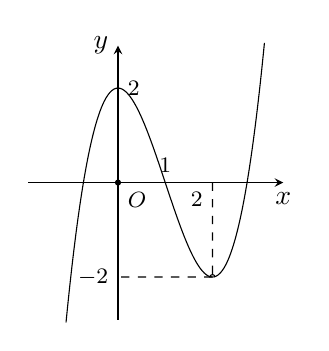
\begin{tikzpicture}[scale=.6,>=stealth]
\draw[->](-1.9,0)--(3.5,0)node[below]{$x$};
\draw[->](0,-2.9)--(0,2.9)node[left]{$y$};
\draw[dashed](2,0)--(2,-2)circle(1.5 pt)--(0,-2);
\node at (1,0) [above ] {\footnotesize $1$};
\node at (2,0) [below left] {\footnotesize $2$};
\node at (0,2) [right] {\footnotesize $2$};
\node at (0,-2) [left] {\footnotesize $-2$};
\draw [fill] (0,0) circle (1.5 pt)node[below right] {\footnotesize $O$};
\draw[smooth,samples=100,domain=-1.1:3.1] plot(\x,{(\x)^3-3*(\x)^2+2});
\end{tikzpicture}
}
\loigiai{
\begin{center}
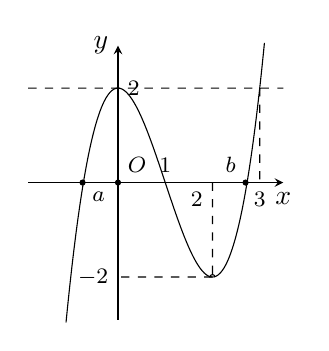
\begin{tikzpicture}[scale=.6,>=stealth]
\draw[->](-1.9,0)--(3.5,0)node[below]{$x$};
\draw[->](0,-2.9)--(0,2.9)node[left]{$y$};
\draw[dashed](2,0)--(2,-2)circle(1.5 pt)--(0,-2) (-1.9,2)--(3.5,2) (3,2)--(3,0);
\node at (1,0) [above ] {\footnotesize $1$};
\node at (2,0) [below left] {\footnotesize $2$};
\node at (0,2) [right] {\footnotesize $2$};
\node at (0,-2) [left] {\footnotesize $-2$};
\node at (3,0) [below] {\footnotesize $3$};
\draw [fill] (0,0) circle (1.5 pt)node[above right] {\footnotesize $O$};
\draw [fill] (-0.75,0) circle (1.5 pt)node[below right] {\footnotesize $a$};
\draw [fill] (2.7,0) circle (1.5 pt)node[above left] {\footnotesize $b$};
\draw[smooth,samples=100,domain=-1.1:3.1] plot(\x,{(\x)^3-3*(\x)^2+2});
\end{tikzpicture}
\end{center}
\begin{itemchoice}
\itemch Dựa vào đồ thị ta thấy $f(x)=0\Leftrightarrow\hoac{&x=a<0\\&x=1\\&x=b>2}$.\\
Từ đó suy ra đồ thị hàm số $g_1(x)$ có $3$  tiệm cận đứng là $ x=a,  x=1, x=b$.
\itemch Dựa vào đồ thị ta thấy $f(x)=2\Leftrightarrow\hoac{&x=0 \text{ nghiệm bội 2}\\&x=b>2}$.\\
Từ đó suy ra đồ thị hàm số $g_2(x)$ có $2$  tiệm cận đứng là $ x=0, x=b$.
\itemch Dựa vào đồ thị ta thấy $f(x)=0\Leftrightarrow\hoac{&x=a<0\\&x=1\\&x=b>2}$.\\
Từ đó suy ra đồ thị hàm số $g_3(x)$ có $2$  tiệm cận đứng là $ x=a, x=b$.
\itemch Dựa vào đồ thị ta thấy $f^2(x)-2f(x)=0\Leftrightarrow\hoac{&f(x)=0\\&f(x)=2}\Leftrightarrow \hoac{&x=a \quad (a<0)\\&x=1\\&x=b\quad  (b>2)\\&x=0 \\&x=3.}$\\
Do đó ta viết $f^2(x)-2f(x)=k (x-a)(x-1)(x-b)x^2(x-3)$.\\
Xét hàm số $  g(x)\dfrac{x^2-x}{\left[f(x)\right]^2-2f(x)} =\dfrac{x(x-1)}{k (x-a)(x-1)(x-b)x^2(x-3)} $.\\
Tập xác định $ \mathscr{D}=\mathbb{R}\backslash\{a;1;b;0;3\} $.\\
Từ đó suy ra đồ thị hàm số $g(x)$ có $4$  tiệm cận đứng là $ x=a,  x=0, x=b, x=3 $ và $1$ tiệm cận ngang là $y=0$.
\end{itemchoice}
}
\end{ex}

\begin{ex}%[Dự án TL12New-4in1-NCT]%[2D1C4-1]
\immini{Cho hàm số $y=f(x)=ax^4+bx^2+c (a\ne 0)$ có đồ thị như hình vẽ.
Xét tính đúng sai của các khẳng định sau.
\choiceTF
{\True Đồ thị hàm số $g(x)=\dfrac{2025(x-2)^3\sqrt{x^2+2026}}{f(x)}$ có $1$ tiệm cận đứng}
{Đồ thị hàm số $g(x)=\dfrac{2025(x+2)^3\sqrt{x^2+2026}}{f(x)}$ có $2$ tiệm cận đứng}
{Đồ thị hàm số $g(x)=\dfrac{2025(x+2)^3\sqrt{x^2+2026}}{f(x)}$ có $1$ tiệm cận ngang}
{\True Đồ thị hàm số $g(x)=\dfrac{2025(x-2)^3\sqrt{x^2+2026}}{f(x)}$ có $2$ tiệm cận ngang}
}{
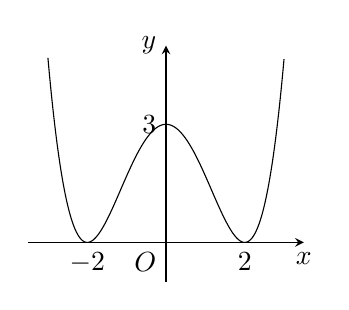
\begin{tikzpicture}[scale=0.5,>=stealth]
\path
(1,1) coordinate (A);
\draw[->](-3.5,0)--(3.5,0)node[below]{$x$};
\draw[->](0,-1)--(0,5)node[left]{$y$};
\draw[smooth,samples=200,domain=-3:3]plot(\x,{3/16*(\x)^4-3/2*(\x)^2+3});
\draw(0,0)node[below left]{$O$} (-2,0)node[below]{$-2$} (2,0)node[below]{$2$} (0,3)node[ left]{$3$};
\end{tikzpicture}}
\loigiai{
Ta có $f(x)=0\Leftrightarrow\hoac{&x=-2\\&x=2.}$\\
Do đó ta viết $f(x)=a(x+2)^2(x-2)^2$.
\begin{itemchoice}
\itemch Xét hàm số  $g(x)=\dfrac{2025(x-2)^3\sqrt{x^2+2026}}{f(x)}=\dfrac{2025(x-2)^3\sqrt{x^2+2026}}{a(x+2)^2(x-2)^2}$.\\
Hàm số $g(x)$ có tập xác định $\mathscr{D}=\mathbb{R}\backslash\{-2;2\}$.\\
Từ đó suy ra đồ thị hàm số $g(x)$ có một tiệm cận đứng là $x=-2$.
\itemch Xét hàm số  $g(x)=\dfrac{2025(x+2)^3\sqrt{x^2+2026}}{f(x)}=\dfrac{2025(x+2)^3\sqrt{x^2+2026}}{a(x+2)^2(x-2)^2}$.\\
Hàm số $g(x)$ có tập xác định $\mathscr{D}=\mathbb{R}\backslash\{-2;2\}$.\\
Từ đó suy ra đồ thị hàm số $g(x)$ có một tiệm cận đứng là $x=2$.
\itemch Xét hàm số  $g(x)=\dfrac{2025(x+2)^3\sqrt{x^2+2026}}{f(x)}=\dfrac{2025(x+2)^3\sqrt{x^2+2026}}{a(x+2)^2(x-2)^2}$.\\
Hàm số $g(x)$ có tập xác định $\mathscr{D}=\mathbb{R}\backslash\{-2;2\}$.\\
Từ đó suy ra đồ thị hàm số $g(x)$ có hai tiệm cận ngang là $y=-\dfrac{2025}{a}$, $y=\dfrac{2025}{a}$.
\itemch Xét hàm số  $g(x)=\dfrac{2025(x-2)^3\sqrt{x^2+2026}}{f(x)}=\dfrac{2025(x-2)^3\sqrt{x^2+2026}}{a(x+2)^2(x-2)^2}$.\\
Hàm số $g(x)$ có tập xác định $\mathscr{D}=\mathbb{R}\backslash\{-2;2\}$.\\
Từ đó suy ra đồ thị hàm số $g(x)$ có hai tiệm cận ngang là $y=-\dfrac{2025}{a}$, $y=\dfrac{2025}{a}$.
\end{itemchoice}
}
\end{ex}

\begin{ex}%[BG-12NEW-4in1, Nguyen Huynh]%[2D1C4-1]
Cho hàm số $y=\dfrac{x-3}{x+1}$ có đồ thị $(C)$. Xét tính đúng sai của các mệnh đề sau
\choiceTF[t]
{ Hàm số đã cho đồng biến trên $\mathbb R\setminus\{1\}$}
{Đồ thị của hàm số chỉ có tiệm cận ngang là $y=3$}
{\True Hai đường tiệm cận của đồ thị hàm số giao nhau tại điểm $I\left(-1;1 \right)$}
{\True Có hai điểm $M$ trên $(C)$ sao cho tiếp tuyến tại $M$ của $(C)$ tạo với hai đường tiệm cận của $(C)$ một tam giác có bán kính đường tròn nội tiếp lớn nhất}
\loigiai{
\begin{itemchoice}
\itemch Ta có $y=1-\dfrac{4}{x+1} \Rightarrow y'=\dfrac{4}{(x+1)^2}>0$ với $x \neq-1$.
\\Do đó hàm số đã cho đồng biến trên từng khoảng xác định.
\itemch Ta có $\lim\limits_{x\to +\infty}f(x)=\lim\limits_{x\to+\infty}\dfrac{x-3}{x+1}=1$ và $\lim\limits_{x\to -\infty}f(x)=\lim\limits_{x\to-\infty}\dfrac{x-3}{x+1}=1$.
Suy ra đường thẳng $y=1$ là tiệm cận ngang của đồ thị $(C)$.
\itemch	Do $\lim\limits_{x\to (-1)^+}f(x)=\lim\limits_{x\to(-1)^+}\dfrac{x-3}{x+1}=-\infty$ nên đường thẳng $x=-1$ là tiệm cận đứng của đồ thị hàm số $y=f(x)$.
\\Vậy $I(-1;1)$ là giao điểm của hai tiệm cận của đồ thị $(C)$.
\itemch  Gọi $M\left(a ; 1-\dfrac{4}{a+1}\right), a \neq-1$.\\
Phương trình tiếp tuyến của $(C)$ tại $M$ là $$d\colon y=\dfrac{4}{(a+1)^2}(x-a)+1-\dfrac{4}{a+1}.$$
Gọi $A$ và $B$ lần lượt là giao điểm của tiếp tuyến $d$ với đường tiệm cận đứng và tiệm cận ngang.\\
Giao điểm của $d$ và tiệm cận đứng là $A\left(-1 ; 1-\dfrac{8}{a+1}\right)$.\\
Giao điểm của $d$ và tiệm cận ngang là $B(2 a+1 ; 1)$.\\
Suy ra $I A=\dfrac{8}{|a+1|}, I B=2|a+1|, A B=\sqrt{4(a+1)^2+\dfrac{64}{(a+1)^2}}$.\\
Vì $\triangle I A B$ vuông tại $I$ nên $S_{\triangle I A B}=\dfrac{1}{2} I A \cdot I B=8$.\\
Nửa chu vi của $\triangle I A B$ là $p=\dfrac{I A+I B+A B}{2}=\dfrac{4}{|a+1|}+|a+1|+\sqrt{(a+1)^2+\dfrac{16}{(a+1)^2}}$.\\
Bán kính đường tròn nội tiếp $\Delta I A B$ là $r=\dfrac{S_{\Delta I A B}}{p}$ nên $r$ lớn nhất khi $p$ nhỏ nhất.\\
Áp dụng bất đắng AM-GM ta có
$$
\dfrac{4}{|a+1|}+|a+1|+\sqrt{(a+1)^2+\dfrac{16}{(a+1)^2}} \geq 2 \sqrt{\dfrac{4}{|a+1|} \cdot|a+1|}+\sqrt{2 \cdot \sqrt{(a+1)^2 \cdot \dfrac{16}{(a+1)^2}}}=4+2 \sqrt{2}.
$$
Suy ra $p \geq 4+2 \sqrt{2}$.\\
$p$ đạt giá trị nhỏ nhất bằng $4+2 \sqrt{2}$ khi $\dfrac{4}{|a+1|}=|a+1| \Leftrightarrow(a+1)^2=4 \Leftrightarrow\hoac{&a=1 \\& a=-3.}$\\
Vậy có hai điểm thỏa mãn yêu cầu bài toán là $M(1 ;-1), M(-3 ; 3)$.
\end{itemchoice}
}
\end{ex}


\Closesolutionfile{ans}

\Opensolutionfile{ans}[ans/ansBTshortans]

\TNSA
\begin{ex}%[2D1C5-7]
Trong mặt phẳng $Oxy$, xét tứ giác tứ giác $ABCD$ có các đỉnh có hoành độ là các số nguyên liên tiếp và nằm trên đồ thị của hàm số $y=\ln x$. Biết diện tích tứ giác $ABCD$ bằng $\ln \dfrac{91}{90}$, tính tổng các chữ số của hoành độ đỉnh xa gốc tọa độ nhất.
\shortans{$6$}
\loigiai{
\immini
{
Giả sử hoành độ của các đỉnh của tứ giác lần lượt là $a$, $a+1$, $a+2$, $a+3$ ($a\in\mathbb{N}^*$) tương ứng với các đỉnh $A$, $B$, $C$, $D$.\\
Khi đó $A(a;\ln a)$, $B(a+1;\ln (a+1))$, $C(a+2;\ln (a+2))$, $D(a+3;\ln (a+3))$.\\
Xét các điểm $M(a;0)$, $N(a+1;0)$, $P(a+2;0)$, $Q(a+3;0)$ thì các tứ giác $ABNM$, $BCPN$, $CDQP$ và $ADQM$ là các hình thang vuông. Khi đó
}
{
\begin{tikzpicture}[line join=round, line cap = round, >=stealth, scale=.8,font=\footnotesize,transform shape]
\pgfmathsetmacro{\a}{ln(2)/ln(1.5)};
\pgfmathsetmacro{\b}{ln(3)/ln(1.5)};
\pgfmathsetmacro{\c}{ln(4)/ln(1.5)};
\pgfmathsetmacro{\d}{ln(5)/ln(1.5)}
\foreach \x/\y/\z/\g in
{
2/\a/A/135,3/\b/B/90,4/\c/C/90,5/\d/D/90,
2/0/M/-90,3/0/N/-90,4/0/P/-90,5/0/Q/-90,0/0/O/-135
}
\draw[fill=black] (\x,\y) circle(1pt) coordinate (\z) ($(\z)+(\g:3mm)$) node{$\z$};
\draw[->] (-.5,0)--(6,0) node[anchor=north]{$x$};
\draw[->] (0,-.5)--(0,4.3) node[anchor=east]{$y$};
\draw[samples=100,domain=.9:5.5] plot(\x,{ln(\x)/ln(1.5)});
\draw (M)--(A) (N)--(B) (P)--(C) (Q)--(D) (A)--(B)--(C)--(D)--(A);
\end{tikzpicture}
}
\begin{eqnarray*}
2S_{ABCD} &=& 2S_{ABNM} + 2S_{BCPN} + 2S_{CDQP} - 2S_{ADQM}\\
&= & \left[ \ln a + \ln (a+1) \right] + \left[ \ln (a+1) + \ln (a+2) \right] + \left[ \ln (a+2) + \ln (a+3) \right] - 3\left[\ln a + \ln (a+3)\right]\\
&= &2\ln \dfrac{(a+1)(a+2)}{a(a+3)}.
\end{eqnarray*}
Kết hợp với $S_{ABCD}=\ln \dfrac{91}{90}$ ta có
$$
\dfrac{(a+1)(a+2)}{a(a+3)} = \dfrac{91}{90} \Leftrightarrow 91a(a+3) = 90(a+1)(a+2)
\Leftrightarrow a^2 + 3a - 180 = 0 \Leftrightarrow \hoac{&a=12\text{ (thỏa mãn)}\\ &a=-15\text{ (loại)}.}
$$
Suy ra đỉnh xa gốc tọa độ nhất là $D(15;\ln 15)$.\\
Vậy $1+5=6$.
}
\end{ex}

\begin{ex}%[2D1C5-7]
Cho hàm số $y=\dfrac{x^2+mx+m^2-2m-4}{x-2}$ có đồ thị $(C)$.
Tìm $m$ để đồ thị $(C)$ có hai điểm cực trị và hai điểm cực trị cách đều đường thẳng $\Delta\colon 2 x+y+1=0$.
\shortans{$-9$}
\loigiai{
Tập xác định $\mathscr{D}=\mathbb{R}\setminus\{2\}$.\\
Ta có  $y'=\dfrac{x^2-4x+4-m^2}{(x-2)^2}$.\\
Dấu của $y'$ là dấu của $g(x)=x^2-4x+4-m^2$.\\
Hàm số có hai điểm cực trị khi và chỉ khi phương trình $g(x)=0$ có hai nghiệm phân biệt khác $2$. Điều kiện tương đương là
$$\heva{& \Delta'=4-4+m^2=m^2>0\\ &
4-8+4-m^2 \neq 0} \Leftrightarrow m \neq 0.$$
Nghiệm của $g(x)=0$ là $x_1=2-m$, $x_2=2+m$, suy ra hai điểm cực trị của đồ thị hàm số là $A(2-m;4-m)$, $B(2+m;4+3m)$.\\
Khoảng cách từ $A$, $B$ đến đường thẳng $\Delta$ lần lượt là $\mathrm{d}(A,\Delta)=\dfrac{|9-3m|}{\sqrt{5}}$ và $\mathrm{d}(B,\Delta)=\dfrac{|9+5m|}{\sqrt{5}}$.\\
Khi đó $$\mathrm{d}(A,\Delta)=\mathrm{d}(B,\Delta)\Leftrightarrow |9-3m|=|9+5m|\Leftrightarrow\hoac{& 9-3m=9+5m\\ &9-3m=-9-5m}\Leftrightarrow\hoac{& m=0 \\ & m=-9.}$$
So với điều kiện $m \neq 0$ ta nhận $m=-9$.\\
Vậy giá trị $m$ cần tìm là $m=-9$.
}
\end{ex}

\begin{ex}%[Dự Án Giảng 12 4 in 1, Lê Văn Toàn]%[2D1C5-7]
Cho hàm số $y=\dfrac{x+2}{x-1}$ có đồ thị $(C)$. Gọi $I$ là giao điểm hai đường tiệm cận của $(C)$. Biết tọa độ điểm $M(a; b)$ có hoành độ dương thuộc đồ thị $(C)$ sao cho $M I$ ngắn nhất. Tính giá trị của $ab-2\sqrt{3}$.
\shortans{$4$}
\loigiai{
Giả sử $M\left(x_0; \dfrac{x_0+2}{x_0-1}\right) \in(C)\left(x_0>0; x_0 \neq 1\right)$.\\
Giao điểm của hai đường tiệm cận của $(C)$ là $I(1; 1)$.\\
Khi đó $M I=\sqrt{\left(1-x_0\right)^2+\left(1-\dfrac{x_0+2}{x_0-1}\right)^2}=\sqrt{\left(1-x_0\right)^2+\dfrac{9}{\left(x_0-1\right)^2}} \geq \sqrt{6}$.\\
Dấu bằng xảy ra khi $$\left(1-x_0\right)^2=\dfrac{9}{\left(x_0-1\right)^2} \Leftrightarrow\left[\begin{array}{l}x_0=1+\sqrt{3} \Rightarrow y_0=1+\sqrt{3} \\ x_0=1-\sqrt{3} \text { (loại).}\end{array}\right.$$
Suy ra $M(1+\sqrt{3}; 1+\sqrt{3}) \Rightarrow(1+\sqrt{3})^2=4+2 \sqrt{3}$.
}
\end{ex}

\begin{ex}%[Dự Án Giảng 12 4 in 1, Lê Văn Toàn]%[2D1C5-6]
Cho hàm số $y=\dfrac{1}{4}x^4-\dfrac{7}{2}x^2$ có đồ thị $(C)$. Tiếp tuyến tại điểm $A$ thuộc $(C)$ cắt $(C)$ tại hai điểm phân biệt $M\left(x_1;y_1\right)$, $N\left(x_2;y_2\right)$ ($M$, $N$ khác $A)$ thỏa mãn $y_1-y_2=6\left(x_1-x_2\right)$. Các điểm $A$ thỏa mãn có tổng các hoành độ là
\shortans{$-3$}
\loigiai{
Gọi $A\left(x_0;y_0\right)\in\,(C)$ là tọa độ tiếp điểm của phương trình tiếp tuyến.\\
Ta có hệ số góc $k=y'\left(x_0\right)=x_0^3-7x_0$.\\
Phương trình tiếp tuyến $y=k\left(x-x_0\right)+y_0=\left(x_0^3-7x_0\right)\left(x-x_0\right)+y_0$.\\
Ta có
\begin{eqnarray*}
&&y_1-y_2=6\left(x_1-x_2\right)\\
&\Leftrightarrow& k\left(x_1-x_0\right)+y_0-\left[k\left(x_2-x_0\right)+y_0\right]=6\left(x_1-x_2\right)\\
&\Leftrightarrow& k\left(x_1-x_2\right)=6\left(x_1-x_2\right)\\
&\Leftrightarrow& k=6\\
&\Leftrightarrow& x_0^3-7x_0=6\\
&\Leftrightarrow& x_0^3-7x_0-6=0\\
&\Leftrightarrow& \hoac{&x_0=3\Rightarrow y_0=-\dfrac{45}{4}\\&x_0=-1\Rightarrow y_0=-\dfrac{13}{4}\\&x_0=-2\Rightarrow y_0=-10.}
\end{eqnarray*}
Khi đó các phương trình tiếp tuyến tương ứng là
$$\hoac{&d_1\colon y=6(x-3)-\dfrac{45}{4}=6x-\dfrac{117}{4}\\&d_2\colon y=6(x+1)-\dfrac{13}{4}=6x+\dfrac{11}{4}\\&d_3\colon y=6(x+2)-10=6x+2.}$$
Phương trình hoành độ giao điểm của $(C)$ với các tiếp tuyến là
$$\hoac{&\dfrac{1}{4}x^4-\dfrac{7}{2}x^2-6x+\dfrac{117}{4}=0\text{ (có 1 nghiệm nên không thỏa)}\\&\dfrac{1}{4}x^4-\dfrac{7}{2}x^2-6x-\dfrac{11}{4}=0\text{ (có 3 nghiệm nên thỏa mãn)}\\&\dfrac{1}{4}x^4-\dfrac{7}{2}x^2-6x-2=0\text{ (có 3 nghiệm nên thỏa mãn).}}$$
Do đó tổng các hoành độ điểm các tiếp điểm là $-1-2=-3$.
}
\end{ex}

\begin{ex}%[2D1C5-5]
\immini
{
Cho hàm số $ f(x)=\dfrac{ax+b}{cx+d} $ (với $ a,\, b,\, c,\, d $ là các số thực) có đồ thị hàm số $ f'(x) $ như hình vẽ. Biết rằng giá trị lớn nhất của hàm số $ y=f(x) $ trên đoạn $ [-3;-2] $ bằng $ 7 $. Giá trị $ f(2) $ bằng
}
{
\begin{tikzpicture}[>=stealth,line join=round,line cap=round,scale=.7]
\def\f(#1){-3/((#1)+1)}
\draw[->] (0,-1)--(0,8)node[right]{$y$};
\draw[->] (-5,0)--(5,0)node[below]{$x$};
\clip (-5,-1) rectangle (5-0.1,8-0.1);
\draw[thick,samples=150,smooth,domain=5:-5] plot(\x,{abs(\f(\x))});
\draw (-1,-1)--(-1,8);
\fill (-1,0)node[below left]{$ -1 $};
\fill (0,0)node[below left]{$O$}circle(1pt);
\end{tikzpicture}
}
\shortans{$3$}
\loigiai{
Ta có $ f'(x)=\dfrac{ad-bc}{(cx+d)^2} $.\\
Từ đồ thị ta có $\heva{&-c+d=0\\ &a d-bc=3d^2}\Leftrightarrow\heva{&c=d\\ &a d-b d=3d^2}\Leftrightarrow\heva{&c=d\\ &a-b=3d.}$ \\
Từ đồ thị $ f'(x)>0 $ nên hàm số $ f(x)=\dfrac{ax+b}{cx+d} $ đồng biến trên $ (-\infty;-1)  $ và $ (-1;+\infty) $.\\
$\Rightarrow\max\limits_{[-3 ; -2]} f(x)=f(-2)=7 \Rightarrow \dfrac{-2a+b}{2c+d} = 7 \Leftrightarrow \dfrac{-2(3d+b)+b}{-2d+d}=7 \Leftrightarrow -6d-b=-7d \Leftrightarrow b=d$.\\
Vậy $f(2)=\dfrac{2a+b}{2c+d}=\dfrac{9d}{3d}=3$.
}
\end{ex}

\begin{ex}%[2D1C5-4]
Cho đường thẳng $d: y=mx+m+2$ ($m$ là tham số) và đường cong $(C): y=\dfrac{2x-1}{x+1}$. Biết rằng khi $m=m_0$ thì $(C)$ cắt $d$ tại hai điểm $A, B$ thỏa mãn độ dài $AB$ ngắn nhất. Tìm $m_0$.
\shortans{$-1$}
\loigiai{Tập xác đinh $\mathscr{D}=\mathbb{R}\setminus \{-1\}$.\\
Phương trình hoành độ giao điểm $mx+m+2=\dfrac{2x-1}{x+1}\Leftrightarrow \dfrac{mx^2+2mx+m+3}{x+1}=0$.\\
Điều kiện cần và đủ để $d$ cắt $C$ tại hai điểm phân biệt là phương trình $mx^2+2mx+m+3=0$ có hai nghiệm phân biệt khác $-1.$ \\
Điều này tương đương
$\heva{&m\ne 0\\&\Delta'=-3m>0\\&3\ne 0}\Leftrightarrow m<0.$\\
Với $m<0$ thì $d$ cắt $C$ tại hai điểm $A(x_1;mx_1+m+2)$ và $B(x_2;mx_2+m+2)$.\\
Theo Vi-et $x_1+x_2=-2$, $x_1x_2=1+\dfrac{3}{m}$. Ta có
\begin{eqnarray*}
AB^2&=& (x_1-x_2)^2+(mx_1-mx_2)^2\\
&=& (m^2+1)((x_1+x_2)^2-4x_1x_2)\\
&=& -\dfrac{12}{m}(m^2+1)\\
&=& -12m-\dfrac{12}{m}\ge 2\sqrt{\dfrac{-12}{m}(-12m)}=24.
\end{eqnarray*}
Dấu bằng xảy ra khi và chỉ khi $m^2=1\Leftrightarrow \heva{&m=1\\&m=-1.}$\\
Kết hợp với $m<0$ ta có $m=-1$ thỏa yêu cầu bài toán.
}
\end{ex}

\begin{ex}%[2D1C5-4]
%[Thi thử L1, chuyên Hùng Vương, Gia Lai 2018]%[2D1G5-4]%[Nguyễn Tài Chung, 12EX-7]
Cho hàm số đa thức bậc ba $y=f(x)$ có đồ thị đi qua các điểm $A(2;4)$, $B(3;9)$, $C(4;16)$. Các đường thẳng $AB, AC, BC$ lại cắt đồ thị tại lần lượt tại các điểm $D$, $E$, $F$ ($D$ khác $A$ và $B$; $E$ khác $A$ và $C$; $F$ khác $B$ và $C$). Biết rằng tổng các hoành độ của $D$, $E$, $F$ bằng $24$. Tính $f(0)$.
\shortans{$6{,}25$}
\loigiai{
Giải sử $f(x)=a(x-2)(x-3)(x-4)+x^2$ ($a\ne 0$). Ta có
$$AB\colon y=5x-6;AC\colon y=6x-8;BC\colon y=7x-12.$$
Hoành độ điểm $D$ là nghiệm của phương trình
\begin{eqnarray*}
& & a\left({x-2}\right)\left({x-3}\right)\left({x-4}\right)=-x^2+5x-6\\
&\Leftrightarrow & a\left({x-2}\right)\left({x-3}\right)\left({x-4}\right)=-\left({x-2}\right)\left({x-3}\right)\\
&\Leftrightarrow & a(x-4)=-1\Rightarrow x=-\dfrac{1}{a}+4.
\end{eqnarray*}
Hoành độ điểm $E$ là nghiệm của phương trình
\begin{eqnarray*}
& & a\left({x-2}\right)\left({x-3}\right)\left({x-4}\right)=-x^2+6x-8\\
&\Leftrightarrow & a\left({x-2}\right)\left({x-3}\right)\left({x-4}\right)=-\left({x-2}\right)\left({x-4}\right)\\
&\Leftrightarrow & a(x-3)=-1\Rightarrow x=-\dfrac{1}{a}+3.
\end{eqnarray*}
Hoành độ điểm $F$ là nghiệm của phương trình
\begin{eqnarray*}
& & a\left({x-2}\right)\left({x-3}\right)\left({x-4}\right)=-x^2+7x-12\\
&\Leftrightarrow & a\left({x-2}\right)\left({x-3}\right)\left({x-4}\right)=-\left({x-3}\right)\left({x-4}\right)\\
&\Leftrightarrow & a(x-2)=-1\Rightarrow x=-\dfrac{1}{a}+2.
\end{eqnarray*}
Theo giả thiết ta có $$-\dfrac{1}{a}+2-\dfrac{1}{a}+3+-\dfrac{1}{a}+4=24\Leftrightarrow -\dfrac{3}{a}=15\Leftrightarrow a=-\dfrac{1}{5}.$$
Do đó $f(0)=a\left({-2}\right)\left({-3}\right)\left({-4}\right)=\dfrac{24}{5}=6{,}25$.}
\end{ex}

\begin{ex}%[2D1C5-4]
Tập hợp tất cả các giá trị thực của tham số $m$ để đồ thị của hàm số $y=x^3-3x^2+2m+1$ cắt trục hoành tại ba điểm phân biệt cách đều nhau là
\shortans{$0{,}5$}
\loigiai{
Phương trình hoành độ giao điểm $x^3-3x^2+2m+1=0\quad (*)$.\\
Giả sử $x_1$; $x_2$; $x_3$ là ba nghiệm của $(*)$.\\
Để $x_1$; $x_2$; $x_3$ cách đều nhau $\Leftrightarrow$ $2x_2=x_1+x_3$ \quad $(1)$\\
Mặt khác\\ $x^3-3x^2+2m+1=(x-x_1)(x-x_2)(x-x_3)$
$=x^3-(x_1+x_2+x_3)x^2+(x_1x_2+x_2x_3+x_3x_1)x-x_1x_2x_3$\\
Nên $x_1+x_2+x_3=3$ $(2)$\\
Từ $(1)$ và $(2)$ suy ra $x_2=1$ $(3)$\\
Thế $(3)$ vào $(*)$ ta được $1-3+2m+1=0 \Leftrightarrow m=\dfrac{1}{2}$.\\
Với $m=\dfrac{1}{2}$ thế vào $(*)$, ta được $x^3-3x^2+2=0 \Leftrightarrow \hoac{&x=1-\sqrt{3}\\&x=1\\&x=1+\sqrt{3}.}$\\
Rõ ràng $3$ nghiệm này cách đều nhau.\\ Vậy $m=\dfrac{1}{2}=0{,}5$ là giá trị cần tìm.}
\end{ex}

\begin{ex}%[2D1C5-4]
Số giao điểm của hai đồ thị hàm số $f(x)=2(m+1)x^3+2mx^2-2(m+1)x-2m$, $\left( m \text{ là tham số khác} -\dfrac{3}{4}\right)$  và $g(x)=-x^4+x^2$ là
\shortans{$4$}
\loigiai{
Phương trình hoành độ giao điểm của hai đồ thị hàm số là
\begin{eqnarray*}
&&-x^4+x^2=2(m+1)x^3+2mx^2-2(m+1)x-2m\\
&\Leftrightarrow & -x^2(x^2-1)=2m(x^3+x^2-x-1)+2x^3-2x\\
&\Leftrightarrow & -x^2(x^2-1)=2m(x^2-1)(x+1)+2x(x^2-1)\\
&\Leftrightarrow &  (x^2-1)\left[x^2+2(m+1)x+2m\right]=0\\
&\Leftrightarrow & \hoac{&x^2-1=0\\&h(x)=x^2+2(m+1)x+2m=0}\\
&\Leftrightarrow & \hoac{&x=\pm 1\\&h(x)=x^2+2(m+1)x+2m=0 \quad(1)}
\end{eqnarray*}
Xét $(1)$ có $\heva{&\Delta =m^2+1>0,\forall m\\&h(-1)=-1\ne 0, \forall m\\&h(1)=4m+3 \ne 0, \forall m \ne -\dfrac{3}{4}.}$\\
$\Rightarrow$ Phương trình $(1)$ luôn có $2$ nghiệm phân biệt khác $\pm 1$.\\
Vậy phương trình đã cho có $4$ nghiệm phân biệt.
}
\end{ex}

\begin{ex}%[2D1C5-4]
\immini{
Cho hàm số bậc ba $y=f(x)$ có đồ thị như hình vẽ bên. Tìm số điểm cực trị của hàm số $g(x)=f\left(\mathrm{e}^x-x\right)$.

}{
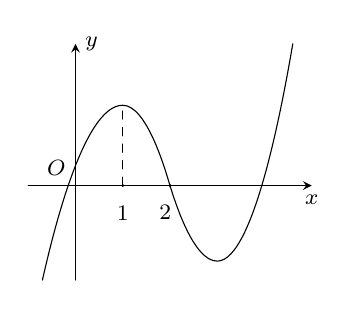
\begin{tikzpicture}[scale=0.6, font=\footnotesize, line join=round, line cap=round,>=stealth]
\def\xmin{-1} \def\xmax{5}
\def\ymin{-2} \def\ymax{3}
\draw[->] (\xmin,0)--(\xmax,0) node [below]{$x$};
\draw[->] (0,\ymin)--(0,\ymax) node [right]{$y$};
\node at (0,0) [above left]{$O$};
\draw[color=black] (-0.7,-2) parabola bend (1,1.7) (2,0) parabola bend (3,-1.6) (4.6,3);
\draw[dashed] (1,0) -- (1,1.7);
\foreach\i/\j/\goc/\diem in{1/0/-90/1,2/0/-100/2}
\fill(\i,\j) circle(1.0pt) node[shift={(\goc:10pt)}]{$\diem$};
\end{tikzpicture}
}
\shortans{$3$}
\loigiai{
Từ đồ thị của hàm số $y=f(x)$ ta có $f'(x)=0\Leftrightarrow\hoac{&x=1\\&x=a>2.}$ \\
Ta có $g'(x)=f'\left(\mathrm{e}^x-x\right)\cdot \left(\mathrm{e}^x-1\right)$ và $g'(x)=0\Leftrightarrow\hoac{&\mathrm{e}^x-1=0\\&\mathrm{e}^x-x=1\\&\mathrm{e}^x-x=a>2}\Leftrightarrow\hoac{&x=0 &&\\&\mathrm{e}^x-x=1&&(1)\\&\mathrm{e}^x-x=a>2.&&(2)}$ \\
Xét hàm số $h(x)=\mathrm{e}^x-x$ trên $\mathbb{R}$, ta có $h'(x)=\mathrm{e}^x-1=0\Leftrightarrow x=0$.\\
Bảng biến thiên của hàm số $y=h(x)$
\begin{center}

\begin{tikzpicture}
\tkzTabInit[nocadre=false,lgt=1.2,espcl=2.5,deltacl=0.6]
{$x$ /0.8, $h'(x)$ /0.8, $h(x)$ /2.5}
{$-\infty$,$0$,$+\infty$}
\tkzTabLine{,-,$0$,+,}
\tkzTabVar{+/$+\infty$, -/$1$,+/$+\infty$}
\end{tikzpicture}
\end{center}
Phương trình $(2)$ có $2$ nghiệm phân biệt khác $0$, phương trình $(1)$ có nghiệm kép $x=0$, do đó phương trình $g'(x)=0$ có $3$ nghiệm trong đó $x=0$ là nghiệm bội $3$.\\
Vậy hàm số $g(x)=f\left(\mathrm{e}^x-x\right)$ có $3$ điểm cực trị.
}
\end{ex}

\begin{ex}%[Mức độ C]%[2D1C5-3]
Cho hàm số $y=f(x)$ có đạo hàm liên tục trên $\mathbb{R}$ và có đồ thị $y=f'(x)$ như hình vẽ. Đặt $g(x)=f(x-m)-\dfrac{1}{2}(x-m-1)^2+2024$, với $m$ là tham số thực. Gọi $S$ là tập hợp các giá trị nguyên dương của $m$ để hàm số $y=g(x)$ đồng biến trên khoảng $(5;6)$. Tổng tất cả các phần tử trong $S$ bằng bao nhiêu?
\begin{center}
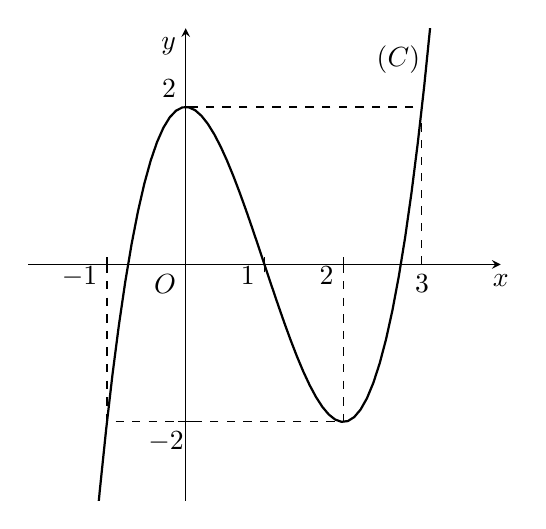
\begin{tikzpicture}[>=stealth]
\draw [->] (-2,0)--(4,0);
\draw [->] (0,-3)--(0,3);
\draw (0,0) node[below left]{$O$};
\draw (4,0) node[below]{$x$};
\draw (0,3) node[below left]{$y$};
\draw (3,0) node[below]{$3$};
\draw (0,2) node[above left]{$2$};
\foreach \x in {-1,1,2,}{\draw (\x,-.1)--(\x,.1) node[below left,black]{$\x$};}
\foreach \y in {-2}{\draw [-] (-.1,\y)--(.1,\y) node[below left,black]{$\y$};}
\clip (-2,-3) rectangle (4,3);
\draw [thick,samples=100] plot[domain=-4:4](\x,{(\x)^3-3*(\x)^2+2});
\draw (3.1,2.9) node[below left]{$(C)$};
\draw[dashed] (2,0)--(2,-2)--(0,-2);
\draw[dashed] (-1,0)--(-1,-2)--(0,-2);
\draw[dashed] (3,0)--(3,2)--(0,2);
\end{tikzpicture}
\end{center}
\shortans{$4$}
\loigiai{Xét hàm số $g(x)=f(x-m)-\dfrac{1}{2}(x-m-1)^2+2019\text{; }g'(x)=f'(x-m)-(x-m-1)$.\\
Cho $g'(x)=0 (1)$.\\
Đặt $x-m=t$, phương trình $(1)$ trở thành $f'(t)-(t-1)=0 \Leftrightarrow f'(t)=t-1 \text{  (2)}$.\\
Nghiệm của phương trình  $(2)$ là hoành độ giao điểm của hai đồ thị hàm số $y=f'(t)$ và $y=t-1$.\\
Đồ thị hai hàm số $y=f'(t)$ và $y=t-1$.
\begin{center}
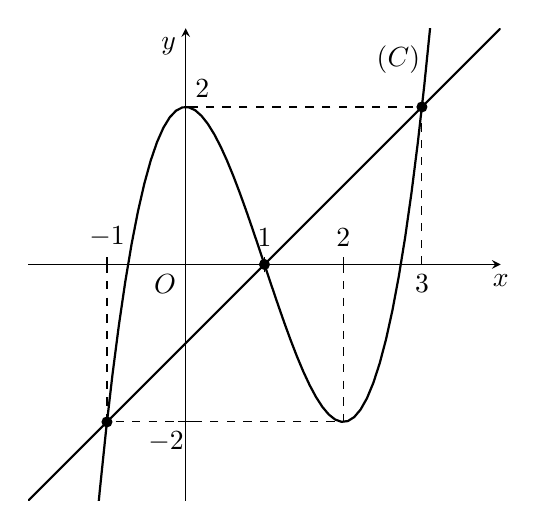
\begin{tikzpicture}[>=stealth]
\draw [->] (-2,0)--(4,0);
\draw [->] (0,-3)--(0,3);
\draw (0,0) node[below left]{$O$};
\draw (4,0) node[below]{$x$};
\draw (0,3) node[below left]{$y$};
\draw (3,0) node[below]{$3$};
\draw (0,2) node[above right]{$2$};
\foreach \x in {-1,1,2,}{\draw (\x,-.1)--(\x,.1) node[above,black]{$\x$};}
\foreach \y in {-2}{\draw [-] (-.1,\y)--(.1,\y) node[below left,black]{$\y$};}
\clip (-2,-3) rectangle (4,3);
\draw [thick,samples=100] plot[domain=-4:4](\x,{(\x)^3-3*(\x)^2+2});
\draw (3.1,2.9) node[below left]{$(C)$};
\draw[dashed] (2,0)--(2,-2)--(0,-2);
\draw[dashed] (-1,0)--(-1,-2)--(0,-2);
\draw[dashed] (3,0)--(3,2)--(0,2);
\draw [thick,samples=100] plot[domain=-4:4](\x,{(\x)-1});
\fill[black] (-1,-2) circle(2pt);
\fill[black] (1,0) circle(2pt);
\fill[black] (3,2) circle(2pt);
\end{tikzpicture}
\end{center}
Từ đồ thị ta có phương trình $(2)$ có nghiệm là $\left[\begin{array}{l}
t=-1\\t=1\\t=3
\end{array}\right. \Rightarrow \left[\begin{array}{l}
x=m-1\\x=m+1\\x=m+3.
\end{array}\right.$\\
Bảng biến thiên
\begin{center}

\begin{tikzpicture}
\tkzTabInit[nocadre=false, lgt=1.5,espcl=3.5]
{$x$/1,$y'$/1,$y$/2}
{$-\infty$,$m-1$,$m+1$,$m+3$,$+\infty$}
\tkzTabLine{,-,0,+,0,-,0,+, }
\tkzTabVar{+/$+\infty$,-/$ $,+/$ $,-/$ $,+/$+\infty$/}
\end{tikzpicture}
\end{center}
Để hàm số $y=g(x)$ đồng biến trên khoảng $(5;6)$ cần $\left[\begin{array}{l}
\begin{cases}
m-1 \leq 5\\m+1 \geq 6
\end{cases}\\
m+3 \leq 5
\end{array}\right. \Leftrightarrow \left[\begin{array}{l}
5 \leq m \leq 6\\
m \leq 2.
\end{array}\right.$\\
Vì $m \in \mathbb{N^{*}}$ mên $m = \{1;2;5;6\}$.\\
Vậy $S=1+2+5+6=14$.
}


\end{ex}

\begin{ex}%[2D1C5-2]
Cho hàm số $f(x)=\dfrac{x^2+5x+2}{2x+1}$. Có tất cả bao nhiêu giá trị nguyên dương của tham số $m$ để bất phương trình $2021f\left(\sqrt{3x^2-18x+28}\right)-m\sqrt{3x^2-18x+28} \geq m+4042$ nghiệm đúng với mọi $x$ thuộc đoạn $[2;4]$?
\shortans{$673$}
\loigiai{
Đặt $u=\sqrt{3 x^2-18 x+28}=\sqrt{3(x-3)^2+1}=\sqrt{3(x-2)(x-4)+4}$.\\
Hàm số $t=3x^2-18x+28$ có $t'=6x-18$ và $t'=0\Leftrightarrow t=3$.\\
Bảng biến thiên của $t$ trên đoạn $[2;4]$ như sau \begin{center}

\begin{tikzpicture}
\tkzTabInit[nocadre=false, lgt=1.2, espcl=2.5, deltacl=0.6]{$x$/0.6,$t'$/0.6,$t$/2}
{$2$, $3$, $4$}
\tkzTabLine {,-,0,+,}
\tkzTabVar{+/$4$, -/$1$, +/$4$}
\end{tikzpicture}
\end{center}
Suy ra $u\in [1;2]$ khi $x\in [2;4]$.\\
Bất phương trình đã cho được viết lại $2021f(u)-mu \geq m+4042 \Leftrightarrow 2021[f(u)-2] \geq m(u+1)$.\\
Ta có $f(x)=\dfrac{x^2+5x+2}{2x+1}$ nên $f(u)-2=\dfrac{u^2+5u+2}{2u+1}-2=\dfrac{u^2+u}{2u+1}$.\\ Do vậy bất phương trình được viết lại thành $\dfrac{2021\left(u^2+u\right)}{2u+1} \geq m(u+1) \Leftrightarrow m \leq \dfrac{2021u}{2u+1}$.\\
Lúc này yêu cầu bài toán tương đương $m \leq \dfrac{2021u}{2u+1},\forall u \in [1;2] \Leftrightarrow m \leq \min\limits_{u \in 1;2]}g(u)$.\\
Xét hàm số $g(u)=\dfrac{2021u}{2u+1}$, $u \in [1;2]$ ta có $g'(u)=\dfrac{2021}{(2u+1)^2}>0$, $\forall u \in [1;2]$.\\
Do vậy hàm số $g(u)$ tăng trên đoạn $[1;2]$.\\
Vì vậy $\min\limits_{u \in [1;2]}g(u)=\dfrac{2021u}{2u+1}=g(1)=\dfrac{2021}{3}$.\\
Kết hợp với $m$ là các số nguyên dương ta được $m \in\{1 ; 2 ; 3 ; \ldots ; 673\}$.\\
Vậy tìm được $673$ số nguyên dương thỏa mãn yêu cầu bài toán.
}
\end{ex}

\begin{ex}%[Dự án Giảng 12 Nhóm Toán & LaTex, Lê Minh Thiện Anh]%[2D1C5-1]
Cho hàm số $f(x)=\dfrac{2-ax}{bx-c}\,(a, b, c \in \mathbb{R}, b \neq 0)$ có bảng biến thiên như sau
\begin{center}

\begin{tikzpicture}
\tkzTabInit[nocadre=false,lgt=1.2,espcl=3]
{$x$/.6,$f'(x)$/.6,$f(x)$/2}
{$-\infty$,$1$,$+\infty$}
\tkzTabLine{ ,+,d,+,}
\tkzTabVar{-/$3$,+D-/$+\infty$/$-\infty$,+/$3$}
\end{tikzpicture}
\end{center}
Tổng $(a+b+c)^2$ thuộc khoảng $\left(0;\dfrac{4}{n}\right)$. Tìm $n$.
\shortans{$9$}
\loigiai{
Ta có $\lim\limits_{x \rightarrow \infty}\dfrac{2-a x}{b x-c}=\dfrac{-a}{b}$, theo giả thiết suy ra $\dfrac{-a}{b}=3 \Leftrightarrow a=-3b$.\\
Hàm số không xác định tại $x=1 \Rightarrow b-c=0 \Leftrightarrow b=c$.\\
Hàm số đồng biến trên từng khoảng xác định nên $f'(x)=\dfrac{ac-2b}{(bx-c)^2}>0$, $\forall x\neq 1$.\\
Suy ra $ac-2b>0 \Leftrightarrow-3b^2-2b>0 \Leftrightarrow-\dfrac{2}{3}<b<0 \Leftrightarrow 0<-b<\dfrac{2}{3}$.\\
Lại có $a+b+c=-3b+b+b=-b$. Suy ra $(a+b+c)^2=b^2 \in\left(0 ; \dfrac{4}{9}\right)$.\\
Vậy tổng $a+b+c$ thuộc khoảng $\left(0;\dfrac{4}{9}\right)$. Vậy $n=9$.
}
\end{ex}

\begin{ex}%[Dự án Giảng 12 Nhóm Toán & LaTex, Lê Minh Thiện Anh]%[2D1C5-1]
Biết hàm số $f(x)=x^3+ax^2+bx+c$ đạt cực đại tại điểm $x=-3$, $f(-3)=28$ và đồ thị của hàm số cắt trục tung tai điểm có tung độ bằng $1$. Tính $S=a^2+b^2-c^2$.
\shortans{$89$}
\loigiai{
Ta có $f'(x)=3 x^2+2 a x+b$; $f''(x)=6x+2a$.\\
Hàm số $f(x)$ đạt cực đại tại điểm $x=-3$ khi và chi khi $\heva{& f'(-3)=0 \\& f''(-3)<0} \Leftrightarrow\heva{& -6a+b=-27 \\ & a<9}$ (1).\\
Mà $f(-3)=28 \Rightarrow 9 a-3 b+c=55(2)$.\\
Ngoài ra, đồ thị của hàm số $f(x)$ cắt trục tung tại điểm có tung độ bằng 1 nên $c=1$ (3).\\
Tù (1), (2), (3) suy ra $\heva{& -6 a+b=-27 \\& 9a-3b+c=55 \\& c=1 \\& a<9} \Leftrightarrow\heva{& a=3 \\& b=-9 \\& c=1 \\ & a<9.}$\\
Do đó $S=3^2+(-9)^2-1^2=89$.
}
\end{ex}

\begin{ex}%[Mức độ 4]giảng 12, Phạm Tiến Long]%[2D1C4-3]
Cho hàm số $f(x)=\dfrac{x^2-2}{x-4}$ có đồ thị $(C)$. Biết đường thẳng $\Delta\colon y=-x+m$ cắt tiệm cận đứng và tiệm cận xiên của $(C)$ lần lượt tại hai điểm $B$, $C$ sao cho tam giác $OBC$ có diện tích bằng $\dfrac{11}{4}$ (với $O$ là gốc tọa độ). Biết $m$ là số nguyên và lớn hơn $1$. Tính giá trị $m^2-1$.
\shortans{$120$}
\loigiai{
Hàm số đã cho có tập xác định là $\mathbb{R}\backslash\{4\}$.\\
Ta có $\lim\limits_{x\to 4^+}f(x)=+\infty$  và 	$\lim\limits_{x\to 4^-}f(x)=-\infty$.\\
Suy ra tiệm cận đứng của $(C)$ là đường thẳng $d\colon x=4$.\\
Mặt khác,	ta có $\begin{aligned}[t]
a&=\lim\limits_{x \rightarrow+\infty} \dfrac{f(x)}{x}=\lim\limits_{x \rightarrow+\infty} \dfrac{x^2-2}{x^2-4x}=1;\\
b&=\lim\limits_{x \rightarrow+\infty}[f(x)-x]=\lim\limits_{x \rightarrow+\infty}\left(\dfrac{x^2-2}{x-4}-x\right)=\lim\limits_{x \rightarrow+\infty} \dfrac{4x-2}{x-4}=4.
\end{aligned}$\\
Ta cũng có $\lim\limits_{x \rightarrow-\infty} \dfrac{f(x)}{x}=1$; $\lim\limits_{x \rightarrow-\infty}[f(x)-x]=4$.
\\
Do đó, đồ thị hàm số có tiệm cận xiên là đường thẳng $d'\colon y=x+4\Leftrightarrow x-y+4=0$.\\
Đường thẳng $\Delta\colon y=-x+m$ cắt hai đường thẳng $d$ và $d'$ lần lượt tại hai điểm $B(4;m-4)$ và $C\left(\dfrac{m-4}{2};\dfrac{m+4}{2}\right)$.\\
Ta có
\begin{itemize}
\item $BC=\sqrt{\left(\dfrac{m-4}{2}-4\right)^2+\left(\dfrac{m+4}{2}-m+4\right)^2}=\sqrt{\dfrac{1}{2}m^2-12m+72}$.
\item $\mathrm{d}(O,\Delta)=\dfrac{|m|\sqrt{2}}{2}$.
\end{itemize} .\\
Theo giả thiết ta có
\begin{eqnarray*}
& & S_{\triangle OBC}=\dfrac{11}{4}\\
&\Leftrightarrow & \dfrac{1}{2}\cdot BC \cdot \mathrm{d}(O,\Delta)=\dfrac{11}{4}\\
&\Leftrightarrow & \dfrac{1}{2}\sqrt{\dfrac{1}{2}m^2-12m+72} \cdot \dfrac{|m|\sqrt{2}}{2}=\dfrac{11}{4}\\
&\Leftrightarrow & \dfrac{1}{4}\cdot \left(\dfrac{1}{2}m^2-12m+72\right)\cdot \dfrac{m^2}{2} =\dfrac{121}{16} \\
&\Leftrightarrow & \dfrac{1}{16}m^4-\dfrac{3}{2}m^3+9m^2-\dfrac{121}{16}=0\\
&\Leftrightarrow & \hoac{&m=1\\&m=11\\&m=6-\sqrt{47}\\&m=6+\sqrt{47}.}
\end{eqnarray*}
Vì $m$ là số nguyên và $m>1$ nên $m=11\Rightarrow m^2-1=120$.
}
\end{ex}

\begin{ex}%[Mức độ 4]giảng 12, Phạm Tiến Long]%[2D1C4-3]
Cho hàm số $f(x)=\dfrac{x^2-4x+5}{x+2}$ có đồ thị $(C)$. Gọi $I$ là giao điểm của tiệm cận đứng và tiệm cận xiên của $(C)$. Đường thẳng $y=m$ (với $m\ne 0$) cắt tiệm cận đứng và tiệm cận xiên của $(C)$ tại hai điểm $A$, $B$ sao cho tam giác $IAB$ có diện tích bằng $32$. Tìm $m$.
\shortans{$-16$}
\loigiai{
Hàm số đã cho có tập xác định là $\mathbb{R}\backslash\{-2\}$.\\
Ta có $\lim\limits_{x\to -2^+}f(x)=+\infty$  và 	$\lim\limits_{x\to -2^-}f(x)=-\infty$.\\
Suy ra tiệm cận đứng của $(C)$ là đường thẳng $d\colon x=-2$.\\
Mặt khác,	ta có $\begin{aligned}[t]
a&=\lim\limits_{x \rightarrow+\infty} \dfrac{f(x)}{x}=\lim\limits_{x \rightarrow+\infty} \dfrac{x^2-4x+5}{x^2+2x}=1;\\
b&=\lim\limits_{x \rightarrow+\infty}[f(x)-x]=\lim\limits_{x \rightarrow+\infty}\left(\dfrac{x^2-4x+5}{x+2}-x\right)=\lim\limits_{x \rightarrow+\infty} \dfrac{-6x+5}{x+2}=-6.
\end{aligned}$\\
Ta cũng có $\lim\limits_{x \rightarrow-\infty} \dfrac{f(x)}{x}=1$; $\lim\limits_{x \rightarrow-\infty}[f(x)-x]=-6$.
\\
Do đó, đồ thị hàm số có tiệm cận xiên là đường thẳng $d'\colon y=x-6$.\\
$I$ là giao điểm của $d$ và $d' \Rightarrow I(-2;-8)$.\\
Đường thẳng $y=m$ cắt hai đường thẳng $d$ và $d'$ lần lượt tại hai điểm $A(-2;m)$ và $B(m+6;m)$.\\
Ta có $\heva{&IA=\sqrt{(m+8)^2}=|m+8|\\&AB=\sqrt{(m+8)^2}=|m+8|}\Rightarrow IA=AB$\quad(1)\\
Dễ thấy đường thẳng $y=m$ vuông góc với $d$ tại $A$.\quad(2)\\
Từ (1) và (2) suy ra tam giác $IAB$ vuông cân tại $A$.\\
Theo giả thiết ta có
\begin{eqnarray*}
& & S_{\triangle IAB}=32\\
&\Leftrightarrow & \dfrac{1}{2}\cdot AB^2=32\\
&\Leftrightarrow & (m+8)^2=64\\
&\Leftrightarrow & m^2+16m=0\\
&\Leftrightarrow & \hoac{&m=0\\&m=-16.}
\end{eqnarray*}
Vì $m\ne 0$  nên suy ra $m=-16$.
}
\end{ex}

\begin{ex}%[Dự án TL12New-4in1-NCT]%[2D1C4-2]
Cho hàm số $y=\dfrac{2x+1}{x-3}$ có đồ thị là $(C)$. Gọi $M$ là điểm bất kì trên đồ thị $(C)$, tìm giá trị nhỏ nhất của tổng khoảng cách từ $M$ đến hai tiệm cận của đồ thị (làm tròn đến $1$ chữ số thập phân).
\shortans{$5{,}3$}
\loigiai{Gọi $M\left(x_M;\dfrac{2x_M+1}{x_M-3}\right),x_M\ne 3$. Các đường tiệm cận ngang, tiệm cận đứng của đồ thị có phương trình lần lượt là $y=2,x=3$.\\
Tổng khoảng cách từ điểm $M$ đến hai tiệm cận là\newline $d=|x_M-3|+\left|\dfrac{2x_M+1}{x_M-3}-2\right|=|x_M-3|+\dfrac{7}{\left|x_M-3\right|}\ge 2\sqrt{7}$.\\
Đẳng thức xảy ra khi và chỉ khi $|x_M-3|=\dfrac{7}{\left|x_M-3\right|}\Leftrightarrow \left[\begin{aligned}&x_M=3+\sqrt{7}\\&x_M=3-\sqrt{7}\end{aligned}\right.$\\
Vậy giá trị giá trị nhỏ nhất của tổng khoảng cách từ $M$ đến hai tiệm cận của đồ thị là $2\sqrt 7\approx5{,}3$.}
\end{ex}

\begin{ex}%[Dự án TL12New-4in1-NCT]%[2D1C4-1]
\immini{
Cho hàm số bậc ba $f(x)$ có đồ thị như hình vẽ. Xác định tổng số các đường tiệm cận đứng và tiệm cận ngang của đồ thị hàm số $ g(x)=\dfrac{\left(x^2-2x-3\right)\sqrt{x+2}}{(x^2-x)\left[f^2(x)+f(x)\right]} $.
\shortans{$7$}
}{
\begin{tikzpicture}[scale=.7,>=stealth]
\draw[->](-2.5,0)--(4,0)node[below]{$x$};
\draw[->](0,-2.5)--(0,3)node[left]{$y$};
\draw[dashed](-1,0)--(-1,-1)circle(1.5 pt)--(0,-1);
\node at (-1,0) [above] {\footnotesize $-1$};
\node at (2,0) [above] {\footnotesize $2$};
\node at (0,-1) [ right] {\footnotesize $-1$};
\draw [fill] (0,0) circle (1.5 pt)node[above right] {\footnotesize $O$};
\draw[smooth,samples=100,domain=-2.1:3.5] plot(\x,{-20/81*((\x)+1.45)*((\x)-2)^2});
\end{tikzpicture}
}
\loigiai{
\begin{center}
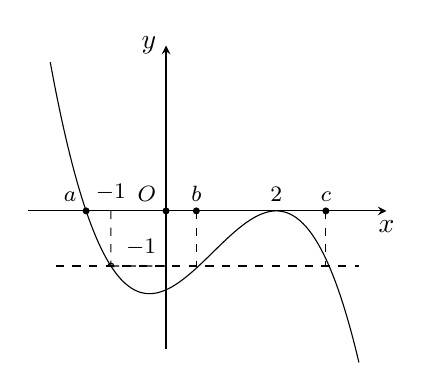
\begin{tikzpicture}[scale=.7,>=stealth]
\draw[->](-2.5,0)--(4,0)node[below]{$x$};
\draw[->](0,-2.5)--(0,3)node[left]{$y$};
\draw[dashed](-1,0)--(-1,-1)circle(1.5 pt)--(0,-1);
\node at (-1,0) [above] {\footnotesize $-1$};
\node at (2,0) [above] {\footnotesize $2$};
\node at (0,-1) [above left] {\footnotesize \footnotesize $-1$};
\draw [fill] (0,0) circle (1.5 pt)node[above left] {\footnotesize $O$};
\draw [fill] (-1.45,0) circle (1.5 pt)node[above left] {\footnotesize $a$};
\draw [fill] (2.9,0) circle (1.5 pt)node[above] {\footnotesize $c$};
\draw [dashed] (-2,-1)--(3.5,-1) (0.55,0)--(0.55,-1)(2.9,0)--(2.9,-1);
\draw [fill] (0.55,0) circle (1.5 pt)node[above ] {\footnotesize $b$};
\draw[smooth,samples=100,domain=-2.1:3.5] plot(\x,{-20/81*((\x)+1.45)*((\x)-2)^2});
\end{tikzpicture}
\end{center}
Dựa vào đồ thị ta thấy $f^2(x)+f(x)=0\Leftrightarrow\hoac{&f(x)=0\\&f(x)=-1}\Leftrightarrow \hoac{&x=a \quad (-2<a<-1)\\&x=2\\&x=-1\\&x=b\quad  (0<b<1)\\&x=c \quad (c>2).}$\\
Do đó ta viết $f^2(x)+f(x)=k x(x-1)(x-a)(x-2)^2(x+1)(x-b)(x-c)$.\\
Xét hàm số $  g(x)=\dfrac{\left(x^2-2x-3\right)\sqrt{x+2}}{(x^2-x)\left[f^2(x)+f(x)\right]}=\dfrac{(x+1)(x-3)\sqrt{x+2}}{k x(x-1)(x-a)(x-2)^2(x+1)(x-b)(x-c)} $.\\
Tập xác định $ \mathscr{D}=[-2;+\infty)\backslash\{0;1;a;2;-1;b;c\} $.\\
Từ đó suy ra đồ thị hàm số $g(x)$ có $6$  tiệm cận đứng là $ x=0, x=1, x=a, x=2, x=b, x=c $ và $1$ tiệm cận ngang là $y=0$.
}
\end{ex}

\begin{ex}%[Dự án TL12New-4in1-NCT]%[2D1C4-1]
\immini{
Cho hàm số $y=ax^4+bx^2+c$ có đồ thị như hình vẽ. Đồ thị hàm số $y=\dfrac{(x^2-4)(x^2+2x)}{\left[f(x)\right]^2+2f(x)-3}$ có bao nhiêu đường tiệm cận đứng?\shortans{$4$}}	{\hspace{0.5cm}
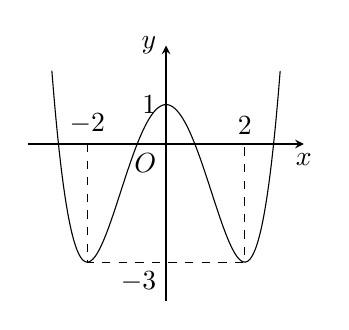
\begin{tikzpicture}[scale=0.5,>=stealth]
\path
(1,1) coordinate (A);
\draw[->](-3.5,0)--(3.5,0)node[below]{$x$};
\draw[->](0,-4)--(0,2.5)node[left]{$y$};
\draw[smooth,samples=200,domain=-2.9:2.9]plot(\x,{1/4*(\x)^4-2*(\x)^2+1});
\draw[dashed](-2,0)--(-2,-3)-- (2,-3)--(2,0);
\draw(0,0)node[below left]{$O$} (-2,0)node[above]{$-2$} (2,0)node[above]{$2$} (0,1)node[ left]{$1$} (0,-3)node[below left]{$-3$};
\end{tikzpicture}}
\loigiai{
\begin{center}
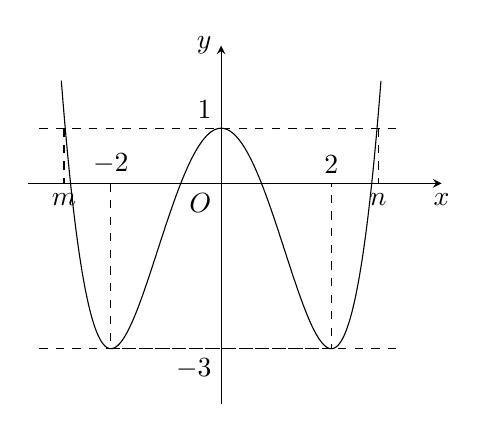
\begin{tikzpicture}[scale=0.7,>=stealth]
\path
(1,1) coordinate (A);
\draw[->](-3.5,0)--(4,0)node[below]{$x$};
\draw[->](0,-4)--(0,2.5)node[left]{$y$};
\draw[smooth,samples=200,domain=-2.9:2.9]plot(\x,{1/4*(\x)^4-2*(\x)^2+1});
\draw[dashed] (-3.3,1)--(3.3,1);
\draw[dashed] (-2.85,1)--(-2.85,0)node[below ]{$m$};
\draw[dashed] (2.85,1)--(2.85,0)node[below ]{$n$};
\draw[dashed] (-3.3,-3)--(3.3,-3);
\draw[dashed](-2,0)--(-2,-3)-- (2,-3)--(2,0);
\draw(0,0)node[below left]{$O$} (-2,0)node[above]{$-2$} (2,0)node[above]{$2$} (0,1)node[above left]{$1$} (0,-3)node[below left]{$-3$};
\end{tikzpicture}
\end{center}
Ta có $\left[f(x)\right]^2+2f(x)-3=0\Leftrightarrow\hoac{&f(x)=1\\&f(x)=-3}\Leftrightarrow\hoac{&x=m \quad (m<-2)\\&x=0\\&x=n\quad (n>2)\\&x=2\\&x=-2.}$\\
Do đó ta viết $\left[f(x)\right]^2+2f(x)-3=kx^2(x+2)^2(x-2)^2(x-m)(x-n)$.\\
Xét hàm số $y=\dfrac{(x^2-4)(x^2+2x)}{\left[f(x)\right]^2+2f(x)-3}=\dfrac{x(x+2)^2(x-2)}{kx^2(x+2)^2(x-2)^2(x-m)(x-n)}$.\\
Hàm số có tập xác định $\mathscr{D}=\mathbb{R}\backslash\{m;-2;0;2;n\}$.\\
Từ đó suy ra đồ thị hàm số đã cho có bốn tiệm cận đứng là $x=0$, $x=2$, $x=m, x=n$.
}

\end{ex}

\begin{ex}%[Dự án TL12New-4in1-NCT]%[2D1C4-1]
\immini
{
Cho hàm số bậc ba $f(x)$  có đồ thị như hình vẽ. Hỏi đồ thị hàm số \break $ g(x)=\dfrac{\left(x^2+4x+3\right)\sqrt{x^2+x}}{x\left[f^2(x)-2f(x)\right]} $ có bao nhiêu đường tiệm cận đứng? 	\shortans{$4$}
}{
\begin{tikzpicture}[scale=.6,>=stealth]
\draw[->](-4.5,0)--(2,0)node[below]{$x$};
\draw[->](0,-2.5)--(0,4)node[left]{$y$};
\draw[dashed](-1,0)--(-1,2)circle(1.5 pt)--(0,2);
\node at (-3,0) [below] {\footnotesize $-3$};
\node at (-1,0) [below] {\footnotesize $-1$};
\node at (0,2) [right] {\footnotesize $2$};
\draw [fill] (0,0) circle (1.5 pt)node[below right] {\footnotesize $O$};
\draw[smooth,samples=100,domain=-4:-0.3] plot(\x,{-(\x)^3-6.5*(\x)^2-12*(\x)-4.5});
\end{tikzpicture}
}
\loigiai{
\begin{center}
\begin{tikzpicture}[scale=.8,>=stealth]
\draw[->](-4.5,0)--(2,0)node[below]{$x$};
\draw[->](0,-2.5)--(0,4)node[left]{$y$};
\draw[dashed](-1,0)--(-1,2)circle(1.5 pt)--(0,2);
\node at (-3,0) [below] {\footnotesize $-3$};
\node at (-1,0) [below] {\footnotesize $-1$};
\node at (0,2) [right] {\footnotesize $2$};
\draw [fill] (0,0) circle (1.5 pt)node[below right] {\footnotesize $O$};
\draw [dashed] (-4.5,2)--(1,2);
\draw [fill](-0.5,0)circle (1.5 pt)node[below right]{$x_3$};
\draw [dashed][fill](-3.8,2)--(-3.8,0)circle (1.5 pt)node[below ]{$x_1$};
\draw [dashed][fill](-1.7,2)--(-1.7,0)circle (1.5 pt)node[below ]{$x_2$};
\draw[smooth,samples=100,domain=-4:-0.3] plot(\x,{-(\x)^3-6.5*(\x)^2-12*(\x)-4.5});
\end{tikzpicture}
\end{center}
Dựa vào đồ thị ta thấy $ f(x)=0\Leftrightarrow \hoac{&x=-3\\&x=x_3\in (-1;0).} $\\
Do đó, ta viết $ f(x)=a(x+3)^2(x-x_3) $.\\
Đồng thời, $ f(x)=2\Leftrightarrow \hoac{&x=x_1\in (-\infty;-3)\\&x=x_2\in (-3;-1)\\&x=-1} $. Do đó, ta viết $ f(x)-2=a(x-x_1)(x-x_2)(x+1) $.\\
Xét hàm số $ g(x)=\dfrac{\left(x^2+4x+3\right)\sqrt{x^2+x}}{x\left[f^2(x)-2f(x)\right]}=\dfrac{(x+1)(x+3)\sqrt{x^2+x}}{a^2x(x+3)^2(x+1)(x-x_1)(x-x_2)(x-x_3)} $.\\
Tập xác định $ \mathscr{D}=(-\infty;x_1)\cup(x_1;-3)\cup(-3;x_2)\cup(x_2;-1)\cup(0;+\infty) $.\\
Từ đó suy ra đồ thị hàm số đã cho có bốn tiệm cận đứng là $ x=0,x=3,x=x_1,x=x_2$.
}
\end{ex}

\begin{ex}%[BG-12NEW-4in1, Nguyen Huynh]%[2D1C4-1]
Gọi $S$ là tập các giá trị nguyên của tham số $m$ sao cho đồ thị hàm số $y = \log (mx^{2} - 2(m+1)x + m+1)$ có hai tiệm cận đứng mà khoảng cách giữa chúng lớn hơn 1. Tích của các phần tử của $S$ bằng bao nhiêu?
\shortans{$-24$}
\loigiai{
Yêu cầu bài toán tương đương với\\ Phương trình $mx^{2} - 2(m+1)x + m+1=0$ có 2 nghiệm phân biệt $x_{1}, x_{2}$ sao cho $|x_{1}-x_{2}|>1$.\\
$\Leftrightarrow \heva{& m \neq 0 \\ & \Delta' > 0 \\ & (x_{1}+x_{2})^{2}-4x_{1}x_{2}>1} \heva{& m\neq 0 \\ & m > -1 \\ & -m^{2}+4m+4 > 0.}$\\
Do $m \in \mathbb{Z}$ nên $S= \{ -1; 1; 2; 3; 4 \}$. Suy ra tích cần tìm bằng $-24$.
}
\end{ex}

\begin{ex}%[BG-12NEW-4in1, Nguyen Huynh]%[2D1C4-1]
Đồ thị hàm số $y=\log\dfrac{x^2-4x+3}{x(x-2)}$ có tất cả bao nhiêu đường tiệm cận?
\shortans{$5$}
\loigiai{
Tập xác định của hàm số là $\mathscr{D}=(-\infty;0)\cup(1;2)\cup(3;+\infty)$.\\
Ta có $\lim\limits_{x\to \pm\infty}\log\dfrac{x^2-4x+3}{x(x-2)}=\log(1)=0$, suy ra đồ thị có tiệm cận ngang là $y=0$.\\
Ta có $\lim\limits_{x\to 0^-}\log f(x)=\lim\limits_{x\to +\infty}\log x=+\infty$, suy ra đồ thị có tiệm cận đứng là $x=0$.\\
Ta có $\lim\limits_{x\to 1^+}\log f(x)=\lim\limits_{x\to 0^+}\log x=-\infty$, suy ra đồ thị có tiệm cận đứng là $x=1$.\\
Ta có $\lim\limits_{x\to 2^-}\log f(x)=\lim\limits_{x\to +\infty}\log x=+\infty$, suy ra đồ thị có tiệm cận đứng là $x=2$.\\
Ta có $\lim\limits_{x\to 3^+}\log f(x)=\lim\limits_{x\to 0^+}\log x=-\infty$, suy ra đồ thị có tiệm cận đứng là $x=3$.
}
\end{ex}

\begin{ex}%[BG-12NEW-4in1, Nguyen Huynh]%[2D1C4-1]
Đồ thị hàm số $y=\log\dfrac{x-2}{x+1}$ có tất cả bao nhiêu đường tiệm cận?
\shortans{$3$}
\loigiai{
Tập xác định của hàm số $\mathscr{D}=(-\infty;-1)\cup(2;+\infty)$.\\
Mà $\lim\limits_{x\to \pm\infty}\log(\dfrac{x-2}{x+1})=\log 1=0$, suy ra $y=0$ là tiệm cận ngang.\\
Mà $\lim\limits_{x\to -1^-}\log\left( \dfrac{x-2}{x+1}\right) =\lim\limits_{x\to -1^-}\log(+\infty)=+\infty$, suy ra $x=-1$ là tiệm cận đứng.\\
Mà $\lim\limits_{x\to 2^+}\log\left( \dfrac{x-2}{x+1}\right) =\lim\limits_{x\to 0^+}\log x=-\infty$, suy ra $x=2$ là tiệm cận đứng.\\
Vậy đồ thị hàm số đã cho có $3$ tiệm cận.
}
\end{ex}

\begin{ex}%[BG-12NEW-4in1, Nguyen Huynh]%[2D1C4-1]
Có tất cả bao nhiêu điểm trên đồ thị hàm số $y=\dfrac{x+1}{x-2}$ sao cho tổng khoảng cách từ điểm đó đến hai đường tiệm cận là nhỏ nhất?
\shortans{$2$}
\loigiai{
Xét $M_0\left(x_0;\dfrac{x_0+1}{x_0-2}\right)$ thuộc đồ thị hàm số.\\
Hai đường tiệm cận của đồ thị hàm số là $x=2$ (tiệm cận đứng) và $y=1$ (tiệm cận ngang).\\
Tổng khoảng cách từ $M_0$ đến hai đường tiệm cận là $$\left|x_0-2\right|+\left|\dfrac{x_0+1}{x_0-2}-1\right|=\left|x_0-2\right|+\dfrac{3}{\left|x_0-2\right|}\geq 2\sqrt{3}.$$
Đẳng thức xảy ra khi và chỉ khi $$\left|x_0-2\right|=\dfrac{3}{\left|x_0-2\right|} \Leftrightarrow |x_0-2|=\sqrt{3} \Leftrightarrow \hoac{x_0=2+\sqrt{3}\\ x_0=2-\sqrt{3}} \Rightarrow \hoac{y_0=1+\sqrt{3}\\ y_0=1-\sqrt{3}.}$$
}
\end{ex}

\begin{ex}%[Mức độ C]%[2D1C3-6]
Ông $A$ muốn xây một cái bể chứa nước lớn dạng một khối hộp chữ nhật không nắp có thể tích bằng $288$cm$^2$. Đáy bể là hình chữ nhật có chiều dài gấp đôi chiều rộng. Hỏi tổng diện tích bể bằng bao nhiêu để chi phí thuê nhân công xây dựng là thấp nhất?

\shortans{$216$}
\loigiai{Theo bài toán, để chi phí thuê nhân công thấp nhất thì ta phải xây dựng bể sao cho tổng diện tích xung quanh và diện tích đáy là nhỏ nhất.\\
Gọi các kích thước của bể lần lượt là $a$(m), $2a$(m), $c$(m).\\
%	\begin{center}
%		\begin{tikzpicture}\def\a{3}\def\b{1}\def\g{30}\def\h{2}
%			\path
%			(0:0) coordinate (A)--++(\g:\b) coordinate (B)--++(0:\a) coordinate (C)--++(\g-180:\b) coordinate (D)
%			\foreach \x in {A,B,C,D}{
%				($(\x)+(90:\h)$) coordinate (\x
%				’)};
%			\draw[dashed] (B’)--(B)--(A)
%			(B)--(C);
%			\draw
%			(A)--(D)--(D’)--(A’)--cycle(A’)--(B’)--(C’)--(D’)(D)--(C)--(C’)			; \end{tikzpicture}
%	\end{center}
Ta có tổng diện tích các mặt cần xây là $S=2a^2+4ac+2ac=2a^2+6ac$.\\
Thể tích bể $V=a \cdot 2a\cdot c=2a^2\cdot c=288 \Rightarrow c=\dfrac{144}{a^2}$.\\
Suy ra $S=2a^2+6a\dfrac{144}{a^2}=2a^2+\dfrac{864}{a}=2a^2+\dfrac{432}{a}+\dfrac{432}{a} \geq 3.\sqrt{2a^2\cdot \dfrac{432}{a}\cdot \dfrac{432}{a}}=216.$\\
Do đó diện tích bể nhỏ nhất là $S=216$.\\
Vậy diện tích bể $S=216$m$^2$ thì chi phí thuê nhân công xây dựng là thấp nhất.}
\end{ex}

\begin{ex}%[Mức độ 4]%[BG12-4IN1, Nguyễn Khánh Trọng]%[2D1C3-6]
\immini[thm]{
Cho một tấm gỗ hình vuông cạnh $200$ cm. Người ta cắt một tấm gỗ có hình một tam giác vuông $ABC$ từ tấm gỗ hình vuông đã cho như hình vẽ bên. Biết $AB=x$ ($0<x<60$ cm) là một cạnh góc vuông của tam giác $ABC$ và tổng độ dài cạnh góc vuông $AB$ với cạnh huyền $BC$ bằng $120$ cm. Tìm $x$ để tam giác $ABC$ có diện tích lớn nhất.
\shortans{$40$}
}{
\begin{tikzpicture}[scale=0.72, font=\footnotesize, line join=round, line cap=round, >=stealth]
\draw[dashed] (0,0)--(4,0)--(0,1)--(0,0);
\draw (4,0)--(5,0)--(5,5)--(0,5)--(0,1);
\node at (0,0.5)[below left] {$x$}; \node at (2,0.5)[above,rotate=-13] {$120-x$}; \node at (2.5,5)[above] {$200$};
\fill (0,0) circle (1.5pt) node[below left]{$A$} (4,0) circle (1.5pt) node[below]{$C$} (0,1) circle (1.5pt) node[left]{$B$};
\end{tikzpicture}
}

\loigiai{
Độ dài cạnh huyền $BC$ là $120-x$.\\
Khi đó độ dài cạnh $AC=\sqrt{BC^2-AB^2}=\sqrt{(120-x)^2-x^2}=\sqrt{14400-240x}$.\\
Diện tích tam giác $ABC$ là $S=\dfrac{1}{2}AB\cdot AC=\dfrac{1}{2}x\sqrt{14400-240x}$.\\
Xét hàm số $f(x)=x\sqrt{14400-240x}$ với $0<x<60$.\\
Ta có $f'(x)=\sqrt{14400-240x}-\dfrac{120x}{\sqrt{14400-240x}}=\dfrac{14400-360x}{\sqrt{14400-240x}}$;\\
$f'(x)=0\Leftrightarrow x=40\in(0;60)$.\\
Bảng biến thiên
\begin{center}

\begin{tikzpicture}
\tkzTabInit[nocadre=false,lgt=1.2,espcl=2.5,deltacl=0.6]
{$x$ /0.6,$f'(x)$ /0.6,$f(x)$ /2}
{$0$,$40$,$60$}
\tkzTabLine{,+,$0$,-,}
\tkzTabVar{-/, +/,-/}
\end{tikzpicture}
\end{center}
Vậy tam giác $ABC$ có diện tích lớn nhất khi $AB=40$ cm.
}
\end{ex}

\begin{ex}%[SGK 12 - Cùng Khám Phá, Mức độ 4]%[BG12-4IN1, Nguyễn Khánh Trọng]%[2D1C3-6]
\immini{Một thùng chứa nhiên liệu gồm phần ở giữa là một hình trụ có chiều dài $h$ mét $(h>0)$ và hai đầu là các nửa hình cầu bán kính $r$ $(r>0)$ (\textit{Hình 1.11}). Biết rằng thể tích của thùng chứa là $144\,000 \pi$ m$^3$. Để sơn mặt ngoài của phần hình cầu cần $20\,000$ đồng cho $1$ m$^2$, còn sơn mặt ngoài cho phần hình trụ cần $10\,000$ đồng cho $1$ m$^2$. Xác định $r$ để chi phí cho việc sơn diện tích mặt ngoài thùng chứa (bao gồm diện tích xung quanh hình trụ và diện tích hai nửa hình cầu) là nhỏ nhất, biết rằng bán kính $r$ không được vượt quá $50$ m.
\shortans{$30$}
}{

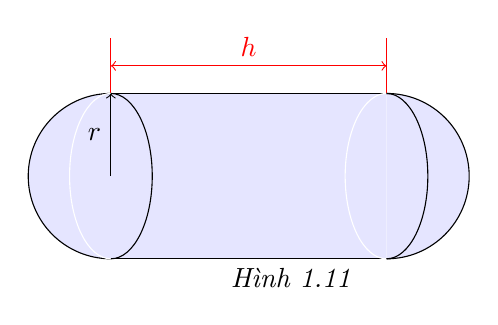
\begin{tikzpicture}[scale=.7]
\draw[white,fill=blue!10] (0,0) rectangle (5,3);
\draw(0,0)--(5,0);
\draw(0,3)--(5,3);
\draw[red](0,3)--(0,4);
\draw[red](5,3)--(5,4);
\draw[fill=blue!10] (5,3) arc(90:-90:1.5);
\draw[fill=blue!10] (0,0) arc(-90:-270:1.5);
\draw[white] (0,3) arc (90:270:0.75 and 1.5);
\draw (0,0) arc (-90:90:0.75 and 1.5);
\draw[white] (5,3) arc (90:270:0.75 and 1.5);
\draw (5,0) arc (-90:90:0.75 and 1.5);
\draw[red,<->] (0,3.5)--(5,3.5) node[midway,above]{$h$};
\draw[->] (0,1.5)--(0,3) node[midway,left]{$r$};
\draw (2,0) node[below right]{\textit{Hình 1.11}};
\end{tikzpicture}
}
\loigiai{
Ta có thể tích của thùng chứa nhiên liệu là $V=\pi \cdot r^2 \cdot h + \dfrac{4}{3} \pi \cdot r^3 = 144\, 000 \pi$ \\
Suy ra $h=\dfrac{(144\,000-\dfrac{4}{3} \cdot r^3)}{r^2}$ \\
Khi đó chi phí sơn diện tích mặt ngoài thùng chứa là
$$2 \pi \cdot r \cdot \dfrac{(144\,000-\dfrac{4}{3} \cdot r^3)}{r^2} \cdot 10^4 + 4 \pi \cdot r^2 \cdot 2 \cdot 10^4 =2 \pi \cdot 10^4 \left( \dfrac{144\,000}{r} + \dfrac{8}{3} r^2 \right). $$
Xét hàm số $f(r)=\dfrac{144\,000}{r} + \dfrac{8}{3} r^2$ với $r \in (0;50]$.\\
Ta có $f'(r)=-\dfrac{144\,000}{r^2} + \dfrac{16}{3} r=\dfrac{16r^3-432\,000}{3r^2}$ và $f'(r)=0 \Leftrightarrow r=30$ m.\\
Bảng biến thiên\\
\begin{center}

\begin{tikzpicture}
\tkzTabInit[nocadre=false,lgt=1.2,espcl=3.5,deltacl=0.6]
{$r$/1,$f'(r)$/1,$f(r)$/3}
{$0$,	$30$,	$50$}
\tkzTabLine{,	-,	$0$,	+}
\tkzTabVar{+/$+\infty$,	-/$7200$,	+/$9546{,}7$}
\end{tikzpicture}
\end{center}
Vậy với $r=30$ m thì chi phí cho việc sơn diện tích mặt ngoài của thùng chứa là nhỏ nhất.
}
\end{ex}

\begin{ex}%[Mức độ 4]%[Dự án giảng 12 - Nguyễn Sĩ Đạt]%[2D1C3-4]
Gọi $S$ là tập hợp các giá trị nguyên của tham số $m\in \left[ 0;2024 \right]$ để bất phương trình ${{x}^{2}}-m+\sqrt{{{\left( 1-{{x}^{2}} \right)}^{3}}}\le 0$ nghiệm đúng với mọi $x\in \left[ -1;1 \right]$. Tập $S$ có bao nhiêu phần tử?
\shortans{$2024$}
\loigiai{
Đặt $t=\sqrt{1-{{x}^{2}}}$, với $x\in \left[ -1;1 \right]\Rightarrow t\in \left[ 0;1 \right]$.\\
Bất phương trình đã cho trở thành ${{t}^{3}}-{{t}^{2}}+1-m\le 0\Leftrightarrow m\ge {{t}^{3}}-{{t}^{2}}+1$.(1)\\
Yêu cầu của bài toán tương đương với bất phương trình (1) nghiệm đúng với mọi $t\in \left[ 0;1 \right]$.\\
Xét hàm số $f\left( t \right)={{t}^{3}}-{{t}^{2}}+1\Rightarrow {f}'\left( t \right)=3{{t}^{2}}-2t$.\\
${f}'\left( t \right)=0\Leftrightarrow \hoac{&t=0\notin \left( 0;1 \right)  \\&t=\frac{2}{3}\in \left( 0;1 \right) .}$\\
Vì $f\left( 0 \right)=f\left( 1 \right)=1$, $f\left( \dfrac{2}{3} \right)=\dfrac{23}{27}$ nên $\underset{\left[ 0;1 \right]}{\mathop{\max }}\,f\left( t \right)=1$.\\
Do đó bất phương trình (1) nghiệm đúng với mọi $t\in \left[ 0;1 \right]$ khi và chỉ khi $m\ge 1$.\\
Mặt khác $m$ là số nguyên thuộc $\left[ 0;2024 \right]$ nên $m\in \left\{ 1;2;3;\ldots;2024 \right\}$.\\
Vậy có $2024$ giá trị của $m$ thỏa mãn bài toán.
}
\end{ex}

\begin{ex}%[Mức độ 4]%[BG12-4IN1, Nguyễn Khánh Trọng]%[2D1C3-4]
Cho hàm số $y=f(x)$ có bảng biến thiên như sau
\begin{center}

\begin{tikzpicture}
\tkzTabInit[nocadre=false,lgt=1.2,espcl=2.5,deltacl=0.6]
{$x$ /0.6,$f'(x)$ /0.6,$f(x)$ /2}
{$0$,  $1$, $3$}
\tkzTabLine{,+,$0$,-}
\tkzTabVar{-/ $8$ ,+/$9$,-/$5$}
\end{tikzpicture}
\end{center}
Gọi $S$ là tập hợp các số nguyên dương $m$ để bất phương trình $f(x) \ge mx^2\left(x^2-2\right)+2m$ có nghiệm thuộc đoạn $[0;3]$. Tìm số phần tử của tập $S$.
\shortans{$9$}
\loigiai{
Bất phương trình đã cho tương đương với $\dfrac{f(x)}{x^4-2x^2+2} \ge m$.\\
Từ bảng biến thiên ta thấy $5 \le f(x) \le 9$ với mọi $x\in [0;3]$.\\
Xét hàm số $g(x)=x^4-2x^2+2$ với $x\in [0;3]$ ta có $g'(x)=4x^3-4x$, $g'(x)=0 \Leftrightarrow \hoac{&x=0\\&x=1.}$\\
Ta lại có $g(0)=2$, $g(1)=1$, $g(3)=65$. Từ đó suy ra $1 \le g(x) \le 65$ với mọi $x\in [0;3]$.\\
Xét hàm số $h(x)=\dfrac{f(x)}{g(x)}$, $x\in [0;3]$. Từ đó ta có đánh giá $\dfrac{5}{65} \le h(x) \le 9$ với mọi $x\in [0;3]$.\\
Từ đó suy ra $\min\limits_{x\in [0;3]} h(x)=\dfrac{5}{65}$ khi $x=3$; $\max\limits_{x\in [0;3]} h(x)=9$ khi $x=1$.\\
Vậy bất phương trình đã cho có nghiệm thuộc đoạn $[0;3]$ khi và chỉ khi $ m \le 9$.\\
Vì $m$ nguyên dương nên có tất cả $9$ giá trị thỏa đề bài.
}
\end{ex}

\begin{ex}%[Mức độ 4]%[BG12-4IN1, Nguyễn Khánh Trọng]%[2D1C3-4]
Cho hàm số $ y=f(x) $ liên tục trên $ \mathbb{R} $ và có bảng biến thiên sau
\begin{center}

\begin{tikzpicture}
\tkzTabInit[lgt=1.5,espcl=2]
{$x$/1,$f’(x)$/.7,$f(x)$/2}
{$-\infty$,$-1$,$1$,$\dfrac{21}{4}$,$7$,$10$,$+\infty$}
\tkzTabLine{ ,+,z,-,z,+,z,-,d,+,z,- }
\tkzTabVar{-/$-\infty$,+/$4$,-/$2$,+/$5$,-/$0$,+/$8$,-/$-\infty$}
\end{tikzpicture}
\end{center}
Gọi $S$ là tập hợp các số nguyên của tham số $m\in[-5;15]$ để bất phương trình $f(x^2-2x)-m\ge 0$ có nghiệm
trên khoảng $\left(-\dfrac{3}{2};\dfrac{7}{2}\right)$. Tìm số phần tử của tập $S$.
\shortans{$10$}
\loigiai{
Đặt $t=x^2-2x$. Với $x\in \left[-\dfrac{3}{2};\dfrac{7}{2}\right] \Leftrightarrow -1 \le (x-1)^2-1 \le \dfrac{21}{4}$ nên $t\in \left[-1;\dfrac{21}{4}\right]$.\\
Xét hàm số $ y=f(t)$, với $t \in \left[-1;\dfrac{21}{4}\right] $.\\
Từ BBT, ta có $\max \limits_{t \in \left[-1;\tfrac{21}{4}\right]}f(t)= f\left(\dfrac{21}{4}\right)=5$.\\
Bất phương trình $f(x^2-2x)-m\ge 0$ có nghiệm
trên khoảng $\left(-\dfrac{3}{2};\dfrac{7}{2}\right)$ khi và chỉ khi
$$\max \limits_{t \in \left[-1;\tfrac{21}{4}\right]}f(t)>m\Leftrightarrow m<5.$$
Vì $m$ nguyên thuộc đoạn $[-5;15]$ nên $m\in\left\{-5;-4;-3;\ldots;3;4\right\}$, suy ra ta có $10$ giá trị thỏa đề bài.
}
\end{ex}

\begin{ex}giảng 12-4in1, Nhật Thiện]%[2D1C3-1]
Giá trị lớn nhất của hàm số $y=\dfrac{x^3+x^2-m}{x+1}$ trên $[0;2]$ bằng $5$. Tham số $m$ nhận giá trị là
\shortans{$-3$}
\loigiai{
Đặt $f(x)=\dfrac{x^3+x^2-m}{x+1}$.\\
Giá trị lớn nhất của $y=f(x)$ trên $[0; 2]$ bằng $5\Leftrightarrow \heva{& f(x)\leq 5,  \forall x\in [0;  2] \\ & \exists x_0\in [0;2]\colon f(x_0)=5.}$\\
\begin{itemize}
\item $f(x)\leq 5$, $\forall x\in [0;2]\Leftrightarrow \dfrac{x^3+x^2-m}{x+1}\leq 5$, $\forall x\in [0;2]$\\
\phantom{$f(x)\leq 5$, $\forall x\in [0;2]$} $\Leftrightarrow m\geq x^3+x^2-5x-5$, $\forall x\in [0;2]$\\
\phantom{$f(x)\leq 5$, $\forall x\in [0;2]$} $\Leftrightarrow m\geq \max\limits_{[0;2]} h(x)$, với $h(x)=x^3+x^2-5x-5$.\\
Ta có $h'(x)=3x^2+2x-5$, $h'(x)=0\Leftrightarrow 3x^2+2x-5=0\Leftrightarrow \hoac{& x=1 \\ & x=-\dfrac{5}{3}\;\text{(loại)}.}$\\
Ta có $h(0)=-5$, $h(2)=-3$, $h(1)=-8$.\\
Suy ra $\max\limits_{[0;2]} h(x)=-3$, $\min\limits_{[0;2]} h(x)=-8$.\\
Vậy $m\geq-3$. \hfill $(1)$
\item $\exists x_0\in [0;2]\colon f(x_0)=5\Leftrightarrow \dfrac{x^3+x^2-m}{x+1}=5$ có nghiệm trên $[0;2]$.\\
\phantom{$\exists x_0\in [0;2]\colon f(x_0)=5$} $\Leftrightarrow m=x^3+x^2-5x-5$ có nghiệm trên $[0;2]$.\\
Theo phần trên, ta suy ra $-8\leq m\leq-3$. \hfill $(2)$
\end{itemize}
Từ $(1)$ và $(2)$ suy ra $m=-3$.
}
\end{ex}

\begin{ex}giảng 12-4in1, Nhật Thiện]%[2D1C2-7]
Gia đình An xây bể hình trụ có thể tích $150$\text{m}$^3$. Đáy bể làm bằng bê tông giá $100000$\text{đ/m}$^2$. Phần thân làm bằng vật liệu chống thấm giá $90000$\text{đ/m}$^2$, nắp bằng nhôm giá $120000$\text{đ/m}$^2$. Hỏi tỷ số giữa chiều cao bể và bán kính đáy là bao nhiêu để chi phí sản xuất bể đạt cực đại? (làm tròn đến hai chữ số thập phân)
\shortans{$2{,}44$}
\loigiai{
Ta có $\pi r^2\cdot h=150 \Rightarrow h=\dfrac{150}{\pi r^2}$.\\
$S_{xq}+S_{đáy}+S_{nắp}=2\pi r\cdot h+\pi r^2+\pi r^2=\dfrac{300}{r}+2\pi r^2$.\\
Chi phí sản xuất bể là $S=\dfrac{300}{r}\cdot 90000+\pi r^2\cdot 220000$.\\
Ta có $S'=-\dfrac{27000000}{r^2}+440000\pi\cdot r$; $S'=0 \Leftrightarrow r=\sqrt[3]{\dfrac{675}{11\pi}}$.\\
Bảng biến thiên
\begin{center}

\begin{tikzpicture}
\tkzTabInit[nocadre=false,lgt=1.2,espcl=2.5,deltacl=0.6]
{$r$ /0.96,$S'$ /0.6,$S$ /3}
{$0$,$\sqrt[3]{\dfrac{675}{11\pi}}$,$+\infty$}
\tkzTabLine{,-,$0$,+,}
\tkzTabVar{+/$+\infty$, -/$S\left(\sqrt[3]{\dfrac{675}{11\pi}}\right)$,+/$+\infty$}
\end{tikzpicture}
\end{center}
Suy ra chi phí sản xuất bể đạt cực trị khi $r=\sqrt[3]{\dfrac{675}{11\pi}}\approx 2{,}44$.
}
\end{ex}

\begin{ex}%[MĐ4]%[2D1C2-6]
Cho hàm số $f(x)=\dfrac{x^2-m(m+1)x+m^3+1}{x-m}$ có đồ thị là $(C_m)$. Điểm $A(a;b)$ vừa là điểm cực đại của $(C_{m_1})$ vừa là điểm cực tiểu của $(C_{m_2})$. Tính $a-b$. \shortans{$1{,}25$}
\loigiai{
Ta có $f(x)=\dfrac{x^2-2mx+m^2-1}{(x-m)^2}$. Suy ra $f'(x)= 0 \Leftrightarrow x=m\pm 1$. Do đó, ta có bảng biến thiên
\begin{center}

\begin{tikzpicture}[font=\footnotesize,>=stealth, scale=1]
\tkzTabInit[nocadre=false,lgt=1.2,espcl=3.5,deltacl=0.6]
{$x$ /0.6,$f'(x)$ /0.6,$f$ /2}
{$-\infty$, $m-1$, $m$, $m+1$, $+\infty$}
\tkzTabLine{,+,0,-,d,-,0,+,}
\tkzTabVar{-/$-\infty$, +/$-m^2+m-2$, -D+/$-\infty$/$+\infty$, -/$-m^2+m+2$,+/$+\infty$}
\end{tikzpicture}
\end{center}
Từ giả thiết, ta có
$$ \heva{&m_1-1=m_2+1\\ &-m_1^2+m_1-2=-m_2^2+m_2+2} \Leftrightarrow \heva{&m_1=m_2+2\\ &4m_2=-6} \Leftrightarrow \heva{&m_1=\frac{1}{2}\\ &m_2=-\frac{3}{2}.} $$
Khi đó $A\left(-\dfrac{1}{2};-\dfrac{7}{4}\right)$, vậy $a-b=-\dfrac{1}{2}+\dfrac{7}{4}=1{,}25$.
}
\end{ex}

\begin{ex}%[MĐ4]%[2D1C2-6]
Cho hàm số $f(x)=\dfrac{x^2+m\left(m^2-1\right)x-m^4+1}{x-m}$, với $m$ là tham số, có đồ thị $(C_m)$. Biết rằng tồn tại duy nhất một điểm vừa điểm cực đại của $(C_{m_1})$ và là cực tiểu của $(C_{m_2})$, tính giá trị của $m_1m_2$.
\shortans{$-1$}
\loigiai{
Ta có $f(x)=x+m^3+\dfrac{1}{x-m}$, $f'(x)=1-\dfrac{1}{(x-m)^2}$. Suy ra $f'(x)=0 \Leftrightarrow x=m\pm 1$. Từ đó, ta có bảng biến thiên
\begin{center}

\begin{tikzpicture}[font=\footnotesize,>=stealth, scale=1]
\tkzTabInit[nocadre=false,lgt=1.2,espcl=2.5,deltacl=0.6]
{$x$ /0.6,$f'(x)$ /0.6,$f(x)$ /2}
{$-\infty$, $m-1$, $m$, $m+1$, $+\infty$}
\tkzTabLine{,+,0,-,d,-,0,+,}
\tkzTabVar{-/$-\infty$, +/$y_1$, -D+/$-\infty$/$+\infty$, -/$y_2$, +/$+\infty$}
\end{tikzpicture}
\end{center}
Ta có đường thẳng đi qua hai điểm cực trị có phương trình
$$ y=\dfrac{\left(x^2+m\left(m^2-1\right)x-m^4+1\right)'}{(x-m)'} \text{ hay } y=2x+m\left(m^2-1\right). $$
Suy ra $y_1=m^3+m-2$ và $y_2=m^3+m+2$. Theo giả thiết, tồn tại một điểm vừa là điểm cực đại của $(C_{m_1})$ và vừa là điểm cực tiểu của $(C_{m_2})$ nên
$$ \heva{&m_1-1=m_2+1\\ &m_1^3+m_1-2=m_2^3+m_2+2} \Leftrightarrow \heva{&m_1=m_2+2\\ &m_2^2+2m_2+1=0} \Leftrightarrow \heva{&m_1=1\\ &m_2=-1.} $$
Vậy $m_1m_2=-1$.
}
\end{ex}

\begin{ex}%[Mức độ C]%[Dự án giảng 12 - Trung Anh]%[2D1C2-5]
Với giá trị nào của tham số $m$ thì hàm số $y=x^4+2mx^2+m^2+m$ có ba điểm cực trị lập thành một tam giác có một góc bằng $120^\circ$? (lấy giá trị xấp xỉ đến hàng phần trăm)
\shortans{$-0{,}69$}
\loigiai
{
Tập xác định của hàm số là $\mathscr{D}=\mathbb{R}$.\\
Ta có $y'=4x^3+4mx = 4x(x^2+m)$.
$$y'=0 \Leftrightarrow 4x(x^2+m)=0 \Leftrightarrow \left[\begin{aligned}&x=0 \\&x^2=-m.\end{aligned}\right.$$
Đồ thị hàm số đã cho có ba điểm cực trị khi phương trình $x^2=-m$ có hai nghiệm phân biệt $x\neq 0$, suy ra $-m >0$ hay $m < 0$.\\
Như vậy, với $m<0$ đồ thị hàm số đã cho có điểm cực trị là $A(0;m^2+m)$, $B\left(\sqrt{-m};m\right)$, $C\left(-\sqrt{-m};m\right)$.\\
Dễ thấy tam giác $ABC$ cân tại $A$. Khi đó $\overrightarrow{AB}=\left(\sqrt{-m};-m^2\right)$, $\overrightarrow{AC} = \left(-\sqrt{-m}; -m^2\right)$.\\
Tam giác $ABC$ có một góc bằng $120^\circ$ nên $\widehat{A} = \left(\overrightarrow{AB},\overrightarrow{AC}\right) = 120^\circ$.\\
Suy ra
\begin{eqnarray*}
\cos\left(\overrightarrow{AB},\overrightarrow{AC}\right) = -\dfrac{1}{2} \Leftrightarrow \dfrac{m^4+m}{m^4-m} = -\dfrac{1}{2} \Leftrightarrow 3m^4+m=0 \Leftrightarrow m(3m^3+1)=0 \Leftrightarrow \left[\begin{aligned}&m=0 \\&m=-\dfrac{1}{\sqrt[3]{3}}.\end{aligned}\right.
\end{eqnarray*}
Kết hợp điều kiện $m<0$ ta được $m=-\dfrac{1}{\sqrt[3]{3}}\approx -0{,}69$ là giá trị thỏa mãn yêu cầu bài toán.
}
\end{ex}

\begin{ex}%[Sách tham khảo, Mức độ C]%[Dự án giảng 12 - Trung Anh]%[2D1C2-5]
Cho hàm số $y=x^4-2m^2x^2+m^2$ có đồ thị $(C)$. Tích các giá trị của $m$ để đồ thị $(C)$ có ba điểm cực trị $A$, $B$, $C$ sao cho bốn điểm $A$, $B$, $C$, $O$ là bốn đỉnh của hình thoi ($O$ là gốc tọa độ).
\shortans{$-0{,}5$}
\loigiai{
Ta có $y'=4x^3-4m^2x$; $y'=0\Leftrightarrow \left[ \begin{aligned}
x=0 \\
x=m^2 \\
\end{aligned} \right. $.\\
Điều kiện để hàm số có ba cực trị là $y'=0$ có ba nghiệm phân biệt $\Leftrightarrow m\ne 0$.\\
Khi đó: $y'=0\Leftrightarrow \left[ \begin{aligned}
x=0 \\
x=\pm m \\
\end{aligned} \right. $.\\
Tọa độ các điểm cực trị là $A(0;m^2)$, $B(m;-m^4+m^2)$, $C(m;-m^4+m^2)$.\\
Ta có $OA\bot BC$, nên bốn điểm $A$, $B$, $C$, $O$ là bốn đỉnh của hình thoi điều kiện cần và đủ là $OA$ và $BC$ cắt nhau tại trung điểm mỗi đoạn\\
$\Leftrightarrow \left\{ \begin{aligned}
{{x}_A}+{{x}_O}={{x}_B}+{{x}_C} \\
{{y}_A}+{{y}_O}={{y}_B}+{{y}_C} \\
\end{aligned} \right. \Leftrightarrow \left\{ \begin{aligned}
0=0 \\
m^2+0=(-m^4+m^2)+(-m^4+m^2) \\
\end{aligned} \right. $\\
$\Leftrightarrow 2m^4-m^2=0 \Leftrightarrow m^2=\dfrac{1}{2} \Leftrightarrow m=\pm \dfrac{\sqrt{2}}{2}$.\\
Vậy $m=\pm \dfrac{\sqrt{2}}{2}$.
}
\end{ex}

\begin{ex}%[Mức độ C]%[Dự án giảng 12 - Trung Anh]%[2D1C2-4]
Hàm số $f(x)=\dfrac{1}{3}x^3-x^2+(m^2-3)x+2018$ có hai điểm cực trị $x_1, x_2$. Tìm giá trị lớn nhất của biểu thức $P=|x_1(x_2-2)-2(x_2+1)|$.
\shortans{$9$}
\loigiai{
Tập xác định $\mathbb{R}$. Đạo hàm $y'=x^2-2x+m^2-3$.\\
Hàm số có hai điểm cực trị $\Leftrightarrow $ phương trình $y'=0$ có hai nghiệm phân biệt $\Leftrightarrow \Delta '>0 \Leftrightarrow 4-m^2>0\Leftrightarrow m \in (-2;2)$.\\
Áp dụng định lí Vi-et ta có $x_1+x_2=2;x_1x_2=m^2-3$.\\
Ta có $P=|x_1x_2-2(x_1+x_2)-2|=|m^2-9|$.\\
Xét hàm số $f(m)=m^2-9, m \in (-2;2)$. Ta có $f'(m)=2m=0\Leftrightarrow m=0$.\\
Bảng biến thiên:
\begin{center}

\begin{tikzpicture}
\tkzTabInit[nocadre=false,lgt=1.5,espcl=2.5,deltacl=0.6]
{$x$ /0.6,$f'(m)$ /0.6,$f(m)$ /2}
{$-2$,$0$,$2$}
\tkzTabLine{,-,0,+,}
\tkzTabVar{+/ $-5$ / , -/ $-9$ /, +/ $-5$ /}
\end{tikzpicture}
\end{center}
Vậy $P_{\max}=9$ đạt tại $m=0$.
}
\end{ex}

\begin{ex}%[Sách tham khảo, Mức độ C]%[Dự án giảng 12 - Trung Anh]%[2D1C2-4]
Gọi $S$ là tập hợp giá trị $m$ là số nguyên để hàm số $y = \dfrac{1}{3}x^3 - \left(m + 1\right)x^2 + \left(m - 2\right)x + 2m - 3$ đạt cực trị tại hai điểm $x_{1}$, $x_{2}$ thỏa mãn $x^2_{1} + x^2_{2} = 18$. Tính tổng các phần tử nguyên thuộc tập $S$.
\shortans{$1$}
\loigiai{Tập xác định $\mathscr{D} = \mathbb{R}$.\\
Ta có $y' = x^2 - 2\left(m + 1\right)x + m - 2$.\\
Xét $y' = 0$ suy ra $x^2 - 2\left(m + 1\right)x + m - 2 = 0\quad (*)$.\\
Để hàm số có hai điểm cực trị khi và chỉ khi phương trình $(*)$ có hai nghiệm phân biệt.
$$\Leftrightarrow \Delta' > 0\Leftrightarrow \left(m + 1\right)^2 - \left(m - 2\right) > 0\Leftrightarrow m^2 + m + 3 > 0\Leftrightarrow \left(m + \dfrac{1}{2}\right)^2 + \dfrac{11}{4} > 0.$$
Dễ thấy $(*)$ luôn có $2$ nghiệm phân biệt với mọi $m$.\\
Khi đó $x_{1}$, $x_{2}$ là nghiệm của phương trình $(*)$.\\
Theo định lý Vi-ét ta có $\heva{&x_{1} + x_{2}  = 2m  +2\\ &x_{1}\cdot x_{2} = m - 2}$\\
Để thỏa mãn bài toán $x_{1}^2 + x_{2}^2  = 18\Leftrightarrow \left(x_{1} + x_{2}\right)^2 - 2x_{1}x_{2} - 18 = 0\quad (**)$.\\
Áp dụng định lý Vi-ét  $(**)$ trở thành
\begin{eqnarray*}
&{ }&\left(2m + 2\right)^2- 2\left(m - 2\right) - 18 = 0\\
&\Leftrightarrow& 4m^2 + 6m - 10 = 0\Leftrightarrow\hoac{& m = 1 \\ &m = - \dfrac{5}{2}.}
\end{eqnarray*}
Do giả thiết suy ra $m = 1$ nên $P = 1$.
}
\end{ex}

\begin{ex}%[BG12, Tran Tony]%[2D1C2-3]
Có bao nhiêu giá trị nguyên của tham số $m$ để hàm số $y=x^6+(m+4)x^5+(16-m^2)x^4+2$ đạt cực tiểu tại $x=0$?
\shortans{$8$}
\loigiai{
Tập xác định $\mathscr D=\mathbb{R}$.\\
Ta có $y'=x^3\cdot\left[6x^2+5(m+4)x+64-4m^2\right]$; $y'=0 \Leftrightarrow\hoac{& x=0\,(\text{bội } 3)\\& 6x^2+5(m+4)x+64-4m^2=0. \quad (*)}$\\
Để hàm số đã cho đạt cực tiểu tại $x=0$ thì $\hoac{& (*) \text{ vô nghiệm}\\& (*) \text{ có nghiệm kép } x=0\\& (*) \text{ có hai nghiệm phân biệt cùng dấu (do } a=6>0).}$
\begin{itemize}
\item \textbf{Trường hợp 1.} $(*)$ vô nghiệm $\Leftrightarrow \Delta<0 \Leftrightarrow 25\cdot (m+4)^2-24\cdot (64-4m^2)<0$.\\
$$\Leftrightarrow 121m^2+200m-1136<0 \Leftrightarrow -4<m<\dfrac{284}{121}.$$
\item \textbf{Trường hợp 2.} $(*)$ có nghiệm kép $x=0 \Leftrightarrow \heva{& \Delta=0\\& x=0.}$\\
$$\Leftrightarrow \heva{& 121m^2+200m-1136=0\\& 64-4m^2=0} \Leftrightarrow \heva{& m=-4 \vee m=\dfrac{284}{121}\\& m=\pm 4} \Leftrightarrow m=-4.$$
\item \textbf{Trường hợp 3.} $(*)$ có hai nghiệm phân biệt khác cùng dấu $\Leftrightarrow \heva{& \Delta>0\\& 6\cdot (64-4m^2)>0.}$\\
$$\Leftrightarrow \heva{& 121m^2+200m-1136>0\\& 64-4m^2>0} \Leftrightarrow \heva{& m\in (-\infty; -4) \cup \left(\dfrac{284}{121}; +\infty\right)\\& m\in (-4;4)} \Leftrightarrow m\in \left(\dfrac{284}{121}; 4\right).$$
\end{itemize}
Do đó $m\in \left[-4; \dfrac{284}{121}\right)\cup \left(\dfrac{284}{121};4\right)$.\\
Lại có $m\in\mathbb{Z}$ nên $m\in \{-4;-3;-2;-1;0;1;2;3\}$.\\
Vậy có $8$ giá trị nguyên của $m$ thỏa mãn yêu cầu bài toán.
}
\end{ex}

\begin{ex}%[BG12, Tran Tony]%[2D1C2-3]
Cho hàm số $y=x^2-2mx-2\ln \left(x^2-2mx+m^2+1\right)$, với $m$ là tham số. Gọi $S$ là tập hợp các giá trị của $m$ để hàm số đã cho đạt cực tiểu tại điểm $x=2$. Tính tổng các phần tử của $S$.
\shortans{$4$}
\loigiai{
Hàm số xác định khi $x^2-2mx+m^2+1>0\Leftrightarrow (x-m)^2+1>0,\,\forall x\in\mathbb{R}$.\\
Do đó hàm số có tập xác định $\mathscr D=\mathbb{R}$.\\
Ta có
\allowdisplaybreaks
\begin{eqnarray*}
y'&=&2x-2m-\dfrac{2(2x-2m)}{x^2-2mx+m^2+1}\\
&=&2(x-m)\left[1-\dfrac{2}{x^2-2mx+m^2+1}\right]\\
&=&\dfrac{2(x-m)(x^2-2mx+m^2-1)}{x^2-2mx+m^2+1}\\
&=&\dfrac{2(x-m)(x-m-1)(x-m+1)}{x^2-2mx+m^2+1}.
\end{eqnarray*}
Bảng xét dấu $y'$
\begin{center}

\begin{tikzpicture}
\tkzTabInit[lgt=1.2,espcl=3]
{$x$ /0.6, $y'$ /0.6}
{$-\infty$,$m-1$,$m$,$m+1$,$+\infty$}
\tkzTabLine{ ,-,$0$,+,$0$,-,$0$, +, }
\end{tikzpicture}
\end{center}
Từ bảng xét dấu $y'$, suy ra hàm số đạt cực tiểu tại các điểm $x=m-1$ và $x=m+1$.\\
Do đó, để hàm số đạt cực tiểu tại điểm $x=2$ thì $\hoac{&m-1=2\\&m+1=2}\Leftrightarrow\hoac{&m=3\\&m=1.}$\\
Suy ra $S=\{1;3\}$.\\
Vậy tổng các phần tử của $S$ là $4$.
}
\end{ex}

\begin{ex}%[BG12, Tran Tony]%[2D1C2-2]
\immini{Cho hàm số $f(x)$ có đạo hàm liên tục trên $\mathbb{R}$. Đồ thị của hàm số $y=f(5-2x)$ như hình vẽ bên. Có bao nhiêu giá trị thực của tham số $m$ thuộc khoảng $(-9;9)$ thoả mãn $2m\in \mathbb{Z}$ và hàm số $y=\left|2f\left(4x^3+1\right)+m-\dfrac{1}{2}\right|$ có $5$ điểm cực trị?
\shortans{$26$}
}
{
\begin{tikzpicture}[>=stealth,line cap=round,line join=round,scale=0.5,font=\footnotesize]
\draw[->] (-1.5,0) -- (5,0) node[below] {\scriptsize $x$};
\draw[->] (0,-4.5) -- (0,4) node[left] {\scriptsize $y$};
\draw (0,0)node[below left]{\scriptsize $O$};
\clip (-1.5,-4.5) rectangle(5,4);
\draw[samples=150,smooth,domain=-1.5:3] plot(\x,{-9/16*(\x)^2*(\x-3)});
\draw[samples=150,smooth,domain=3:5] plot(\x,{2.37*(\x)^3-22.21*(\x)^2+63.88*(\x)-55.67});
\draw[dashed] (2,0)|-(0,2.25) (4,0)|-(0,-3.8);
\draw[fill] (0,-3.8) circle(1pt) node[left]{$-4$} (2,0) circle(1pt) node[below]{$2$} (4,0) circle(1pt) node[above]{$4$} (0,2.25) circle(1pt) node[left]{$\dfrac{9}{4}$} (2,2.25) circle(1pt) (4,-3.8) circle(1pt) (0,0) circle(1pt);
\end{tikzpicture}
}
\loigiai{
Dựa vào đồ thị, ta thấy hàm số 	$y=f(5-2x)$ có ba điểm cực trị là $0$, $2$, $4$.\\
Suy ra phương trình $y'=-2f'(5-2x)=0$ có ba nghiệm phân biệt $0$, $2$, $4$ $\Rightarrow \hoac{& 5-2x=0\\& 5-2x=2\\ & 5-2x=4}\Leftrightarrow \hoac{& x=\dfrac{5}{2}\\ & x=\dfrac{3}{2}\\ & x=\dfrac{1}{2}.}$\\
Suy ra hàm số $f(x)$ có ba điểm cực trị là $\dfrac{1}{2}$, $\dfrac{3}{2}$, $\dfrac{5}{2}$.\\
Ta có bảng biến thiên của hàm số $y=f(x)$ như sau
\begin{center}

\begin{tikzpicture}
\tkzTabInit[espcl=2.5,lgt=1.5]
{$x$/1,$f'(x)$/0.7,$f(x)$/1.8}
{$-\infty$,$\dfrac{1}{2}$, $\dfrac{3}{2}$,$\dfrac{5}{2}$,$+\infty$}
\tkzTabLine{,-,0,,+,0,-,0,+}
\tkzTabVar{+/$+\infty$,-/$-4$,+/$\dfrac{9}{4}$,-/$0$,+/$+\infty$}
\end{tikzpicture}
\end{center}
Đặt $t=4x^3+1$, dễ thấy hàm số $u$ đồng biến trên $\mathbb{R}$ và ứng với mỗi giá trị $t$, ta tìm được duy nhất giá trị $x$.\\
Ta cũng có bảng biến thiên của hàm số $y=f\left(4x^3+1\right)$ như sau
\begin{center}

\begin{tikzpicture}
\tkzTabInit[espcl=2.5,lgt=2.5]
{$x$/0.7,$f\left(4x^3+1\right)$/2}
{$-\infty$,$a$, $b$, $c$,$+\infty$}
\tkzTabVar{+/$+\infty$,-/$-4$,+/$\dfrac{9}{4}$,-/$0$,+/$+\infty$}
\end{tikzpicture}
\end{center}
Từ đó suy ra hàm số $f\left(4x^3+1\right)$ có ba điểm cực trị.\\
Suy ra hàm số $y=2f\left(4x^3+1\right)+m-\dfrac{1}{2}$ có ba điểm cực trị.\\
Do đó, hàm số $y=\left|2f\left(4x^3+1\right)+m-\dfrac{1}{2}\right|$ có $5$ điểm cực trị khi và chỉ khi phương trình $$2f\left(4x^3+1\right)+m-\dfrac{1}{2}=0$$ có hai nghiệm bội lẻ phân biệt.\\
Xét phương trình $2f\left(4x^3+1\right)+m-\dfrac{1}{2}=0\Leftrightarrow -\dfrac{m}{2}+\dfrac{1}{4}=f\left(4x^3+1\right)$.\quad $(1)$\\
Dựa vào bảng biến thiên của $f\left(4x^3+1\right)$, phương trình $(1)$ có hai nghiệm bội lẻ khi và chỉ khi
$$\hoac{&-\dfrac{m}{2}+\dfrac{1}{4}\ge \dfrac{9}{4}\\ & -4<-\dfrac{m}{2}+\dfrac{1}{4}\le 0}\Leftrightarrow \hoac{& m\le -4\\ & \dfrac{1}{2}\le m<\dfrac{17}{2}}\Leftrightarrow \hoac{& 2m\le -8\\ & 1\le 2m<17.}$$
Do $m\in (-9;9)$ nên $2m\in (-18;18)$ và $2m\in \mathbb{Z}$ nên $2m\in \{-17;-16;\ldots;-8;1;2;\ldots;16\}$.\\
Vậy có $26$ giá trị $m$ cần tìm.
}
\end{ex}

\begin{ex}%[BG12, Tran Tony]%[2D1C2-2]
\immini{
Cho hàm số bậc bốn $y=f(x)$ có đồ thị hàm số $y=f'(x)$ như hình vẽ. Gọi $m$, $n$ lần lượt là số điểm cực đại và số điểm cực tiểu của hàm số $$h(x)=2f\left(\left|3-x\right|\right)+1.$$ Tính $T=2m+3n$
\shortans{$13$}
}
{
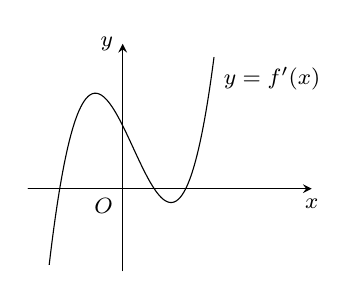
\begin{tikzpicture}[line join = round, line cap = round,>=stealth,font=\footnotesize,scale=0.8]
\def \xmin{-1.5};
\def \xmax{3};
\def \ymin{-1.3};
\def \ymax{2.3};
\draw[->] (\xmin,0) -- (\xmax,0) node[below] {$x$};
\draw[->] (0,\ymin) -- (0,0) node[below left] {$O$} -- (0,\ymax) node[left] {$y$};
\clip (\xmin+0.1,\ymin+0.1) rectangle (\xmax+0.1,\ymax-0.1);
\draw[smooth, samples=100] plot[domain=-1.5:1.45] (\x,{2*(\x+1)*(\x-0.5)*(\x-1)}) node[below right] {$y=f'(x)$};
\end{tikzpicture}
}
\loigiai{
Dựa vào đồ thị ta thấy $f'(x)=0\Leftrightarrow \hoac{& x=a<0 \\ & x=b>0\\& x=c>b.}$\\
Ta có $h'(x)=2\dfrac{(x-3)}{|x-3|}f'\left(|3-x|\right)$, $h'(x)=0\Leftrightarrow \hoac{& |3-x|=b \\ & |3-x|=c}\Leftrightarrow \hoac{& x=3+b \\ & x=3-b\\& x=3+c\\& x=3-c.}$\\
Bảng xét dấu đạo hàm
\begin{center}

\begin{tikzpicture}[line join = round, line cap = round,>=stealth,font=\footnotesize,scale=1]
\tkzTabInit[nocadre=false,lgt=1.2,espcl=2.5,deltacl=0.6]
{$x$ /0.6, $h'(x)$ /0.6}
{$-\infty$,$3-c$,$3-b$,$3$,$3+b$,$3+c$,$+\infty$}
\tkzTabLine{ ,-,z,+,z,-,d,+,z,-,z,+, }
\end{tikzpicture}
\end{center}
Dựa vào bảng xét dấu của $h'(x)$ ta thấy hàm số $y=h(x)$ có $2$ điểm cực đại và $3$ điểm cực tiểu.\\
Vậy $T=2m+3n=13$.
}
\end{ex}

\begin{ex}%[Mức độ 4]%[2D1C2-1]
Giả sử $A$, $B$ là hai điểm cực trị của đồ thị hàm số $y=x^3+a x^2+b x+c$ và đường thẳng $(AB)$ đi qua gốc tọa độ. Giá trị nhỏ nhất $\mathrm{P}_{\min}$ của $P=a b c+a b+c$ bằng $-\dfrac{m}{n}$ (với $\dfrac{m}{n}$ là phân số tối giản, $m;n$ nguyên dương). Tính $m+n$.
\shortans{$34$}
\loigiai
{
Tập xác định $\mathscr{D}=\mathbb{R}$.\\
$f'(x)=3x^2+2ax+b$.\\
Điều kiện để hàm số có hai điểm cực trị là $f'(x)=0$ có hai nghiệm phân biệt $\Rightarrow a^2-3b>0$.\\
Lấy $f(x)$ chia cho $f'(x)$, ta có $f(x)=f'(x)\left(\dfrac{1}{3}x+\dfrac{1}{9}a\right)+\left(\dfrac{2}{3}b-\dfrac{2}{9}\right)x+c-\dfrac{1}{9}ab$.\\
Suy ra, đường thẳng qua hai cực trị là $(AB): y=\left(\dfrac{2}{3} b-\dfrac{2a^2}{9}\right) x+c-\dfrac{a b}{9}$.\\
Do $(AB)$ qua gốc $O$ nên $c-\dfrac{a b}{9}=0\Leftrightarrow a b=9c$.\\
Khi đó $P=a b c+a b+c=9c^2+10c=\left(3c+\dfrac{5}{3}\right)^2-\dfrac{25}{9}\ge-\dfrac{25}{9},\forall c\in\mathbb{R}$.\\
Vậy $\mathrm{P}_{\text{min}}=-\dfrac{25}{9}$ khi $\heva{&c=-\dfrac{5}{9}\\&a b=-5.}$\\
Suy ra $m+n=34$.
}
\end{ex}

\begin{ex}%[Mức độ 4]%[2D1C2-1]
Cho hàm số $y=f(x)$ có đúng ba điểm cực trị là $-2;-1;0$ và có đạo hàm liên tục trên $\mathbb{R}$. Khi đó hàm số $y=f\left(x^2-2x\right)$ có bao nhiêu điểm cực trị?
\shortans{$7$}
\loigiai
{
Do hàm số $y=f(x)$ có đúng ba điểm cực trị là $-2;-1;0$ và có đạo hàm liên tục trên $\mathbb{R}$ nên $f'(x)=0$ có ba nghiệm là $x=-2;x=-1;x=0$.\\
Đặt $g(x)=f\left(x^2-2x\right)\Rightarrow g'(x)=(2x-2)\cdot f'\left(x^2-2x\right)$. \\
Vì $f'(x)$ liên tục trên $\mathbb{R}$ nên $g'(x)$ cũng liên tục trên $\mathbb{R}$.\\
Do đó những điểm $g'(x)$ có thể đổi dấu khi đi qua các điểm thỏa mãn
$$\hoac{&{2 x-2=0}\\&
{x^2-2 x=-2}\\&
{x^2-2 x=-1}\\&
{x^2-2 x=0}}
\Leftrightarrow\hoac{&x=1\\&x=0\\&x=2.}$$
Vậy hàm số $g(x)$ có ba điểm cực trị.
}
\end{ex}

\begin{ex}%[CD12-CTST, Mức độ 4]%[2D1C1-5]
\immini{Mặt cắt ngang của một máng dẫn nước là một hình thang cân có độ dài đáy bé bằng độ dài cạnh bên và bằng $a$ (cm) không đổi (Hình vẽ). Gọi $\alpha$ là một góc của hình thang cân tạo bởi đáy bé và cạnh bên $\left(\dfrac{\pi}{2} \leq \alpha<\pi\right)$. Tìm $\alpha$ để diện tích mặt cắt ngang của máng lớn nhất.}
{\begin{tikzpicture}[>=stealth,line join=round,line cap=round,font=\footnotesize,scale=0.6]
\path
(0,0) coordinate (D)
(4,0) coordinate (C)
($(C)!1!-120:(D)$) coordinate (B)
($(D)!1!120:(C)$) coordinate (A)
;
\draw(A)--(D)node[pos=0.5,left]{$a$};
\draw(D)--(C)node[pos=0.5,below]{$a$};
\draw(C)--(B)node[pos=0.5,right]{$a$};
\draw[fill=cyan!80!blue] (A)--(B)--(C)--(D)--(A);
\draw (A)--(D)--(C)--(B);
\draw pic[draw, angle radius=3mm, angle eccentricity=1.5]{ angle = B--C--D};
\node at ($(C)+(100:0.75)$){\small $\alpha$};
%			\draw (1.8,-0.7)node[below]{$\text{Hình 5}$ };
\end{tikzpicture}}
Hàm số $S(\alpha)$ mô tả diện tích mặt cắt ngang theo góc $\alpha$ có bảng biến thiên như sau
\begin{center}

\begin{tikzpicture}
\tkzTabInit[lgt=1.5, espcl=4]
{$x$/.6,$S'(\alpha)$/0.6,$S(\alpha)$/3}{$0$,$a$,$\pi$}
\tkzTabLine{,+,0,-,}
\tkzTabVar{-/$0$,+/$b$,-/$1$}
\end{tikzpicture}
\end{center}
Tính $a\cdot b$. (làm tròn đến hàng phần trăm)
\shortans{$2{,}72$}
\loigiai{
\immini{Vì $ABCD$ là hình thang cân nên $\heva{&\widehat{A}=\widehat{B}\\&\widehat{C}=\widehat{D}=\alpha.}$\\
$\widehat{A}+\widehat{B}+\widehat{C}+\widehat{D}=2\pi$.\\
$2\widehat{A}+2\alpha=2\pi$ hay $\widehat{A}=\pi-\alpha$.\\
$DH=AD\sin A=a\cdot \sin \left(\pi-a\right)=a\sin \alpha$.\\
$\begin{aligned}[t]AB&=DC+2AH\\
&=a+2a\cos \left(\pi-a\right)\\
&=a-2a\cos \alpha\\
&=a\left(1-2\cos \alpha\right).
\end{aligned}$}
{\begin{tikzpicture}[>=stealth,line join=round,line cap=round,font=\footnotesize,scale=0.6]
\path
(0,0) coordinate (D)
(4,0) coordinate (C)
($(C)!1!-120:(D)$) coordinate (B)
($(D)!1!120:(C)$) coordinate (A)
($(A)!(D)!(B)$) coordinate (H)
;
\draw(A)--(D)node[pos=0.5,left]{$a$};
\draw(D)--(C)node[pos=0.5,below]{$a$};
\draw(C)--(B)node[pos=0.5,right]{$a$};
\draw[fill=cyan!80!blue] (A)--(B)--(C)--(D)--(A);
\draw(A)--(D)--(C)--(B) (D)--(H);
\foreach \x/\y in {A/90,B/90,C/-90,D/-90,H/90}
\draw[fill=black] (\x) circle (1.1pt) + (\y:0.5cm) node{$\x$};
\end{tikzpicture}}
\noindent Diện tích mặt cắt ngang
\begin{eqnarray*}
S&=&\dfrac{1}{2}\cdot \left(AB+CD\right)\cdot DH\\
&=&\dfrac{1}{2}\left[a\left(1-2\cos \alpha\right)+a\right]a\sin \alpha\\
&=&a^2\left(1-\cos \alpha\right)\sin \alpha.
\end{eqnarray*}
$S'(\alpha)=2a^2\sin \dfrac{3\alpha}{2}\sin \dfrac{\alpha}{2}$.\\
$S'(\alpha)=0\Leftrightarrow \hoac{&\alpha=\dfrac{2k\pi}{3}\\&\alpha=2k\pi.}\, (k\in \mathbb{Z})$.\\
Vì $\dfrac{\pi}{2}\leq \alpha<\pi$ nên  $x=\dfrac{2\pi}{3}$.\\
$S\left(\dfrac{2\pi}{3}\right)=\dfrac{3\sqrt{3}}{4}$.\\
$S\left(\dfrac{\pi}{2}\right)=1$.\\
Bảng biến thiên
\begin{center}

\begin{tikzpicture}
\tkzTabInit[lgt=1.5, espcl=4]
{$x$/1,$S'(\alpha)$/0.6,$S(\alpha)$/3}{$0$,$\dfrac{2\pi}{3}$,$\pi$}
\tkzTabLine{,+,0,-,}
\tkzTabVar{-/$0$,+/$\dfrac{3\sqrt{3}}{4}$,-/$1$}
\end{tikzpicture}
\end{center}
Vậy $a\cdot b =\dfrac{2\pi}{3}\cdot \dfrac{3\sqrt{3}}{4}\approx2{,}72$.
}
\end{ex}

\begin{ex}%[CD12-CTST, Mức độ 4]%[2D1C1-5]
\immini{

Người ta muốn thiết kế một lồng nuôi cá có bề mặt hình chữ nhật bao gồm phần mặt nước có diện tích bằng $54$ m$^2$ và phần đường đi xung quanh với kích thước (đơn vị: m) như Hình vẽ.
Khi kích thước $a$ thay đổi trong khoảng $(3;+\infty)$ thì giá trị hàm số mô tả diện tích lối đi theo kích thước $a$ sẽ giảm đến giá trị $S_0$ rồi tăng lên. Xác định giá trị $S_0$.

}
{\begin{tikzpicture}[>=stealth,line join=round,line cap=round,font=\footnotesize,scale=0.75]
\path
(0,0) coordinate (A)
(5,0) coordinate (B)
(0,4) coordinate (D)
($(D)+(B)-(A)$) coordinate (C)
($(B)+(-0.5,0)$) coordinate (M)
($(B)+(0,0.5)$) coordinate (N)
($(A)+(1,0)$) coordinate (H)
($(A)+(0,0.5)$) coordinate (T)
($(C)+(-0.5,0)$) coordinate (Q)
($(C)+(0,-0.5)$) coordinate (P)
($(D)+(1,0)$) coordinate (R)
($(D)+(0,-0.5)$) coordinate (S)
($(T)+(H)-(A)$) coordinate (A')
($(M)+(N)-(B)$) coordinate (B')
($(Q)+(P)-(C)$) coordinate (C')
($(R)+(S)-(D)$) coordinate (D')
($(D)+(0,0.5)$) coordinate (x)
($(C)+(0,0.5)$) coordinate (y)
($(D)+(-0.5,0)$) coordinate (u)
($(A)+(-0.5,0)$) coordinate (v)
($(A)+(0,-0.5)$) coordinate (x')
($(H)+(0,-0.5)$) coordinate (y')
($(M)+(0,-0.5)$) coordinate (u')
($(B)+(0,-0.5)$) coordinate (v')
($(C)+(0.5,0)$) coordinate (x'')
($(P)+(0.5,0)$) coordinate (y'')
($(N)+(0.5,0)$) coordinate (u'')
($(B)+(0.5,0)$) coordinate (v'')
;
\draw[fill=cyan!20!brown](A)--(B)--(C)--(D)--(A);
\draw[fill=cyan!90!blue](A')--(B')--(C')--(D')--(A');
\draw(D)--(x) (C)--(y)(D)--(u)(A)--(v)(A)--(x')(H)--(y')(M)--(u')(B)--(v')(C)--(x'') (P)--(y'') (N)--(u'') (B)--(v'');
\draw[<->] (x)--(y)node[pos=0.5,above]{$a$};
\draw[<->] (u)--(v)node[pos=0.5,left]{$b$};
\draw[<->] (x')--(y')node[pos=0.5,below]{$2$};
\draw[<->] (u')--(v')node[pos=0.5,below]{$1$};
\draw[<->] (u'')--(v'')node[pos=0.5,right]{$1$};
\draw[<->] (x'')--(y'')node[pos=0.5,right]{$1$};
%			\draw (2.2,-0.5)node[below]{$\text{Hình 8}$ };
\end{tikzpicture}}
\shortans{$42$}
\loigiai{
Gọi $x$, $y$ lần lượt là độ dài, rộng của mặt nước. Điều kiện $x$, $y>0$.\\
Phần mặt nước có diện tích bằng $54$ m$^2$ nên ta có $$x\cdot y=54.\, \hfill(*)$$
Theo đề bài ta có $x=a-3$, $y=b-2$.\\
Từ $(*)$ suy ra $$(a-3)(b-2)=54\Rightarrow b=\dfrac{54}{a-3}+2=\dfrac{2a+48}{a-3}.$$
Diện tích lối đi là \begin{eqnarray*}
S(a)&=&a\cdot b-x\cdot y\\
&=&ab-54\\
&=&a\cdot \dfrac{2a+48}{a-3}-54\\
&=&\dfrac{2a^2+48a}{a-3}-54.
\end{eqnarray*}
$S'(a)=\dfrac{2a^2-12a-144}{\left(a-3\right)^2}$;\\
$S'(a)=0\Leftrightarrow \hoac{&a=-6\\&a=12.}$\\
Bảng biến thiên
\begin{center}

\begin{tikzpicture}
\tkzTabInit[nocadre=false, lgt=1.2, espcl=2.4]{$a$ /0.7,$S'(a)$ /0.7,$S(a)$ /2.5}{$0$,$3$,$12$,$+\infty$}
\tkzTabLine{,-,d,-,$0$,+,}
\tkzTabVar{+/$-54$  ,-D+/$-\infty$/$+\infty$,-/$42$,+/$+\infty$}
\end{tikzpicture}
\end{center}
Vậy $S_0=42$.
}
\end{ex}

\begin{ex}%[Mức độ 3]%[Dự án giảng new 4in1, Trần Quang Thạnh]%[2D1C1-4]
Tính tổng tất cả các nghiệm của phương trình $\log_{3}\dfrac{x^{2}+x+3}{2x^{2}+4x+5}=x^{2}+3x+2 $.
\shortans{$1$}
\loigiai{Xét phương trình $\log_{3}\dfrac{x^{2}+x+3}{2x^{2}+4x+5}=x^{2}+3x+2$. $\qquad(*)$\\
Điều kiện xác định $ \heva{&\dfrac{x^{2}+x+3}{2x^{2}+4x+5}>0\\ &2x^{2}+4x+5\neq 0}\Leftrightarrow \forall x\in\mathbb{R} $.\\
Ta có
\begin{eqnarray*}
(*)&\Leftrightarrow& \log_{3} (x^{2}+x+3)-\log_{3}(2x^{2}+4x+5)=(2x^{2}+4x+5)-(x^{2}+x+3)\\
&\Leftrightarrow& (x^{2}+x+3)+\log_{3} (x^{2}+x+3)=\log_{3}(2x^{2}+4x+5)+(2x^{2}+4x+5).
\end{eqnarray*}
Xét hàm số $ f(t)=t+\log_{3}t $ trên khoảng $ (0;+\infty ) $.\\
Ta có cơ số $ 3>1 $ và hàm số $ y=t $ đồng biến nên $ f(t) $ đồng biến trên khoảng $ (0;+\infty) $.\\
Do đó $ f(x^{2}+x+3)=f(2x^{2}+4x+5)\Leftrightarrow x^{2}+x+3=2x^{2}+4x+5\Leftrightarrow x^{2}+3x+2=0\Leftrightarrow\hoac{&x=-1\\ &x=2.} $\\
Do đó $ x=-1 $, $ x=2 $ là các nghiệm của phương trình.\\
Vậy tổng các nghiệm của phương trình là $1$.
}
\end{ex}

\begin{ex}%[Mức độ 4]%[Dự án giảng new 4in1, Trần Quang Thạnh]%[2D1C1-4]
Có bao nhiêu số nguyên dương $y>4$ sao cho tồn tại số thực $x\in(1;6)$ thỏa mãn $4(x-1)\mathrm{e}^x=y(\mathrm{e}^x+xy-2x^2-3)$?
\shortans{$14$}
\loigiai{
\allowdisplaybreaks
\begin{eqnarray*}
&&	4(x-1)\mathrm{e}^x=y(\mathrm{e}^x+xy-2x^2-3)\\
&\Leftrightarrow& 4(x-1)\mathrm{e}^x-y(\mathrm{e}^x+xy-2x^2-3)=0.
\end{eqnarray*}
Xét hàm số $y=f(x)=4(x-1)\mathrm{e}^x-y(\mathrm{e}^x+xy-2x^2-3)$ liên tục trên $[1;6]$ có
\allowdisplaybreaks
\begin{eqnarray*}
f'(x)&=&4\mathrm{e}^x+4(x-1)\mathrm{e}^x-y(\mathrm{e}^x+y-4x)\\
&=&(\mathrm{e}^x+y)(4x-y).
\end{eqnarray*}
\noindent
Cho $f'(x)=0\Leftrightarrow x=\dfrac{y}{4}$.\\
Do $x\in(1;6)$ nên hàm số $y=f(x)$ sẽ tồn tại điểm cực trị $x=\dfrac{y}{4}$ khi $ y\in (4;24)$.\\
Từ đó ta có cơ sở chia các trường hợp như sau
\begin{itemize}
\item Trường hợp 1: $y\ge 24$.
\begin{center}

\begin{tikzpicture}
\tkzTabInit[nocadre=false,lgt=1.2,espcl=2.5,deltacl=0.6]
{$x$/0.7,$f'(x)$/0.7,$f(x)$/2}
{$1$,$6$}
\tkzTabLine{,-,}
\tkzTabVar{+/$f(1)$,-/$f(6)$}
\end{tikzpicture}
\end{center}
Ta có $\heva{&f(1)=-y(\mathrm{e}+y-5)\\&f(6)=20\mathrm{e}^6-y(\mathrm{e}^6+6y-75).}$\\
Điều kiện cần và đủ để tồn tại $x$ là
$$\heva{&f(6)<0\\&f(1)\cdot f(6)<0}\Rightarrow f(1)>0.$$
Mặt khác ta thấy $-y(\mathrm{e}+y-5)<0,\;\forall y\ge 24$ (vô lí) nên loại.
\item Trường hợp 2: $4<y<24$.
\begin{center}

\begin{tikzpicture}
\tkzTabInit[nocadre=false,lgt=1.2,espcl=2.5,deltacl=0.6]
{$x$/0.7,$f'(x)$/0.7,$f(x)$/2}
{$1$,$\tfrac{y}{4}$,$6$}
\tkzTabLine{,-,z,+,}
\tkzTabVar{+/$f(1)$,-/$f\left(\tfrac{y}{4}\right)$,+/$f(6)$}
\end{tikzpicture}
\end{center}
Do $f(1)<0$ nên để tồn tại nghiệm $x\in(1;6)$ thì $f(6)>0$
\allowdisplaybreaks
\begin{eqnarray*}
&\Leftrightarrow&20\mathrm{e}^6-y(\mathrm{e}^6+6y-75>0\\
&\Leftrightarrow&\heva{&-6y^2-(\mathrm{e}^6-75)y+20\mathrm{e}^6>0\\&y\in\mathbb{N}^*;\;y\in(4;24)}\\
&\Leftrightarrow&y\in\{5;6;\ldots;18\}.
\end{eqnarray*}
\end{itemize}
Vậy có tất cả $14$ giá trị nguyên dương $y$ thỏa đề bài.
}
\end{ex}

\begin{ex}%[Đề Tham khảo 2021, Mức độ 4]%[Dự án giảng new 4in1, Trần Quang Thạnh]%[2D1C1-4]
Có bao nhiêu số nguyên $a ~(a\ge2)$ sao cho tồn tại số thực $x$ thỏa mãn $\left(a^{\log x}+2\right)^{\log a}=x-2$?
\shortans{$8$}
\loigiai{
Với $x>0$ đặt $y=a^{\log x}+2>0$ ta được $y^{\log a}=x-2\Leftrightarrow x=a^{\log y}+2$. \\
Từ đó ta có $y=a^{\log x}+2$ và $x=a^{\log y}+2$.\\
Do $a\ge2$ nên $f(t)=a^t+2$ đồng biến trên $\mathbb R$.\\ Giả sử $x\ge y$ thì $f(y)\ge f(x)$, suy ra $y\ge x$ tức là $x=y$. Tương tự $x\le y$ cũng có $x=y$.\\
Vì thế chỉ xét phương trình $x=a^{\log x}+2$ với $x>0$ hay $x-x^{\log a}=2$.\\
Ta phải có $x>2$ và $x>x^{\log a}\Leftrightarrow 1>\log a\Leftrightarrow a<10$.\\
Ngược lại $a<10$ thì xét hàm số liên tục $g(x)=x-x^{\log a}-2=x^{\log a}\left(x^{1-\log a}-1\right)-2$ có $\lim\limits_{x\to+\infty}g(x)=+\infty$ và $g(2)<0$ nên $g(x)$ sẽ có nghiệm trên $(2;+\infty)$. \\
Do đó các số $a\in \{2,3,\ldots,9\}$ đều thỏa mãn.
}
\end{ex}

\begin{ex}%[Mức độ 4]%[Dự án giảng new 4in1, Trần Quang Thạnh]%[2D1C1-3]
Có bao nhiêu giá trị nguyên của tham số $m$ trên khoảng $(-100;100)$ sao cho hàm số $y=\dfrac{-\mathrm{e}^x+3}{\mathrm{e}^x+m}$ nghịch biến trên khoảng $(0;+\infty)$?
\shortans{$101$}
\loigiai{
Điều kiện: $\mathrm{e}^x\neq-m$.\\
Ta có $y'=\mathrm{e}^x\cdot\dfrac{-m-3}{\left(\mathrm{e}^x+m\right)^2}$.\\
Ta có $\heva{&\mathrm{e}^x>0\\&\mathrm{e}^x\in(1;+\infty)}$, $\forall x\in(0;+\infty)$ và khi $x\in(0;+\infty)$ thì $\mathrm{e}^x \in (1;+\infty)$.\\
Suy ra hàm số $y$ nghịch biến trên khoảng $(0;+\infty)$ khi và chỉ khi
$$\heva{&-m-3<0\\&-m\notin(1;+\infty)}\Leftrightarrow\heva{&m >-3\\&m\geq-1}\Leftrightarrow m\geq-1.$$
Vì $\heva{&m\in\mathbb{Z}\\&m\in(-100;100)}$ nên $m\in\left\{-1;0;1;\ldots;99\right\}$.\\
Suy ra có $101$ giá trị của $m$ thỏa mãn.
}
\end{ex}

\begin{ex}%[Mức độ 4]%[Dự án giảng new 4in1, Trần Quang Thạnh]%[2D1C1-3]
Có bao nhiêu giá trị nguyên của tham số $a$ trên đoạn $[-100; 100]$ để hàm số $f(x)=\dfrac{(a+1)\ln x-6}{\ln x-3a}$ nghịch biến trên khoảng $(1; \mathrm{e})$?
\shortans{$198$}
\loigiai{
Ta có $f'(x)=(\ln x)' \cdot \dfrac{-3a^2-3a+6}{(\ln x-3a)^2}=\dfrac{1}{x}\cdot \dfrac{-3a^2-3a+6}{(\ln x-3a)^2}.$\\
Với
$1<x<\mathrm{e}$ thì  $0<\ln x<1$.\\
Do đó hàm số $f(x)$ nghịch biến trên khoảng $(1; \mathrm{e})$ khi và chỉ khi
$$\heva{&-3a^2-3a+6<0\\&3a\notin(0; 1)}\Leftrightarrow\heva{&\hoac{&a <-2\\&a>1}\\&\hoac{&a\leq 0\\&a\geq\dfrac{1}{3}}}\Leftrightarrow\hoac{&a <-2\\&a>1.}$$
Vì $m\in [-100;100]$ nên $m\in \{-100;-99;\ldots;-3;1;\ldots;100\}$.\\
Vậy có $198$ giá trị nguyên của tham số $a$ để hàm số đã cho nghịch biến trên khoảng $(1; \mathrm{e})$.
}
\end{ex}

\begin{ex}%[BG12new-4in1, Trần Hoà]%[2D1C1-2]
\immini{
Cho hàm số $f(x)$ có đồ thị như hình vẽ bên. Xét $x\in \left(0;\dfrac{\pi}{2}\right)$, biết hàm số $f(\sin x)$ nghịch biến trên khoảng $(a;b)$. Khi đó giá trị lớn nhất của $|a-b|$ bằng bao  nhiêu? (kết quả làm tròn đến hàng phần phần trăm).
\shortans[]{$0{,}52$}
}{
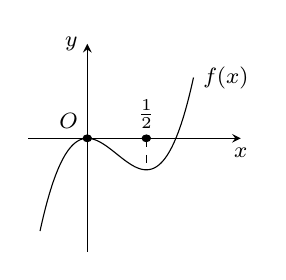
\begin{tikzpicture}[>=stealth,font=\footnotesize,yscale=1.2, xscale=1.5]
\draw[->] (-0.5,0) -- (1.3,0) node[below] {$x$};
\draw[->] (0,-1.2) -- (0,1) node[left] {$y$};
\filldraw (0,0) node[above left=-0.1] {$O$} circle (1pt);
\draw[smooth,samples=100,domain=-0.4:0.9] plot(\x,{(16/3)*(\x)^3-4*(\x)^2}) node[right]{$f(x)$};
\filldraw (0.5,0) node[above] {$\frac{1}{2}$} circle (1pt);
\draw[dashed] (0.5,0) -- (0.5,-0.33);
\end{tikzpicture}
}
\loigiai{
Từ đồ thị của hàm số $f(x)$, suy ra
$$f'(x)<0\Leftrightarrow 0<x<\dfrac{1}{2};\qquad f'(x)>0\Leftrightarrow\hoac{&x<0\\ &x>\dfrac{1}{2}.}$$
Đặt $g(x)=f(\sin x)$, ta có $g'(x)=\cos x\cdot f'(\sin x)$. Xét trên khoảng $(0;\pi)$:
$$g'(x)<0\Leftrightarrow\hoac{&\cos x>0\ \text{và}\ f'(\sin x)<0\\ &\cos x<0\ \text{và}\ f'(\sin x)>0}\Leftrightarrow \hoac{&0<x< \dfrac{\pi}{2}\ \text{và}\ f'(\sin x)<0\qquad \qquad\ (1)\\ &\dfrac{\pi}{2}<x<\pi\ \text{và}\ f'(\sin x)>0.\qquad \qquad (2)}$$
Ta có
{\allowdisplaybreaks
\begin{align*}
&(1)\Leftrightarrow \heva{&0<x<\dfrac{\pi}{2}\\ &0<\sin x<\dfrac{1}{2}}\Leftrightarrow 0<x<\dfrac{\pi}{6}.\\
&(2)\Leftrightarrow \heva{&\dfrac{\pi}{2}<x<\pi\\ &\hoac{&\sin x<0\\ &\sin x>\dfrac{1}{2}}}\Leftrightarrow \dfrac{\pi}{2}<x<\dfrac{5\pi}{6}.
\end{align*}}
Vậy hàm số nghịch biến trên khoảng $\left(0;\dfrac{\pi}{6}\right)$. Suy ra $a=0$, $b=\dfrac{\pi}{6}$. Vậy $a+b\approx 0{,}52$.
}
\end{ex}

\begin{ex}%[2D1C1-1]
Cho hàm số $y= f(x)$ có đạo hàm $f'(x)=(x-1)(x-2)$.
Biết hàm số $y = f(x-x^2)$ nghịch biến trên khoảng có dạng $\left(\dfrac{a}{b};+\infty\right)$ với $\dfrac{a}{b}$ là tối giản và $b>0$. Giá trị của biểu thức $a^2+b^2$ bằng bao nhiêu?
\shortans[]{$5$}
\loigiai{
Đặt $y = g(x) = f(x-x^2) \Rightarrow g'(x) = f'(x-x^2) \cdot (x-x^2)' = (1-2x)f'(x-x^2)$.\\
Khi đó
\allowdisplaybreaks
\begin{eqnarray*}
g'(x) = 0
&\Leftrightarrow& \hoac{&1-2x=0\\&f'(x-x^2) =0 }\\
&\Leftrightarrow&  \hoac{& 1-2x=0\\ & x-x^2 =1\\& x-x^2 =2}\\
&\Leftrightarrow&  x = \dfrac{1}{2}.
\end{eqnarray*}
Với $x< \dfrac{1}{2}$ thì $\heva{&1-2x>0\\& f'\left[ - \left( x- \dfrac{1}{2}\right)^2 + \dfrac{1}{4}  \right] >0  } $ nên $g'(x)>0$.\\
Với $x> \dfrac{1}{2}$ thì $\heva{&1-2x<0\\& f'\left[ - \left( x- \dfrac{1}{2}\right)^2 + \dfrac{1}{4}  \right] >0  } $ nên $g'(x)<0$.\\
Hay hàm số $g(x) = f(x-x^2)$ nghịch biến trên khoảng $\left( \dfrac{1}{2}; + \infty \right) $.\\
Suy ra $a=1$, $b=2$ nên $a^2+b^2=5$.
}
\end{ex}

\begin{ex}%[2D1C5-5]
\immini{Cho hàm số $y=f(x)$ có đạo hàm trên $\mathbb{R}$. Biết rằng hàm số $y=f'(x)$ có đồ thị như hình vẽ bên. Hỏi đồ thị hàm số $y=f(2x-3)$ cắt đường thẳng $y=-3x+2$ tại nhiều nhất bao nhiêu điểm?
}
{
\begin{tikzpicture}[>=stealth,line join=round,line cap=round,font=\scriptsize,scale=0.7]
\draw [->] (-2.5,0)--(2.5,0)node[below]{$ x $};
\draw [->] (0,-3.5)--(0,2)node[left]{$ y $};
\draw [fill=black] (0,0)node[below left]{$ O $}circle(1pt) (-1,0)node[below left]{$ -1 $}circle(1pt) (1,0)node[below]{$ 1 $}circle(1pt) (0,1)node[left]{$ 1 $}circle(1pt) (0,-1)node[right]{$ -1 $}circle(1pt) (0,-3)node[right]{$-3$} circle (1pt) ;
\draw [smooth,domain=-2.1:2.1] plot(\x,{-(\x)^3+3*(\x)-1});
\draw[dashed] (-1,0)|-(0,-3) (1,0)|-(0,1);
\clip (-2.5,-3.5) rectangle (2.5,2.2);
\end{tikzpicture}
}
\shortans{$4$}
\loigiai{
Phương trình hoành độ giao điểm của hai đồ thị hàm số $y=f(2x-3)$ và $y=-3x+2$
$$f(2x-3)=-3x+2\Leftrightarrow f(2x-3)+3x-2=0.$$
Đặt $g(x)=f(2x-3)+3x-2$, ta có $g'(x)=2f'(2x-3)+3=0\Leftrightarrow f'(2x-3)=-\dfrac{3}{2}$.\\
Dựa vào đồ thị, đường thẳng $y=-\dfrac{3}{2}$ cắt đồ thị $f'(x)$ tại ba điểm phân biệt nên phương trình $f'(2x-3)=-\dfrac{3}{2}$ cũng có ba nghiệm phân biệt, giả sử ba nghiệm đó lần lượt là $a$, $b$, $c$ với $a<b<c$.\\
Ta có bảng biến thiên
\begin{center}
\begin{tikzpicture}
\tkzTabInit[nocadre=false,lgt=1.2,espcl=2.5,deltacl=.6]
{$x$/1,$g'(x)$/0.6,$g(x)$/2}
{$-\infty$, $a$, $b$, $c$, $+\infty$}
\tkzTabLine{,+,0,-,0,+,0,-,}
\tkzTabVar{-/,+/,-/,+/,-/}
\end{tikzpicture}
\end{center}
Dựa vào bảng biến thiên, suy ra phương trình $g(x)=0$ có tối đa $4$ nghiệm hay đồ thị hàm số $y=f(2x-3)$ cắt đường thẳng $y=-3x+2$ tại nhiều nhất $4$ điểm.
}
\end{ex}


\Closesolutionfile{ans}

\newpage
\begin{center}
    \bfseries\faGg~\faGg~\faGg~BẢNG ĐÁP ÁN TRẮC NGHIỆM~\faGg~\faGg~\faGg
\end{center}
\inputansbox{8}{ans/ansBTchoice}
\inputansbox[3]{2}{ans/ansBTchoiceTF}
\inputansbox{6}{ans/ansBTshortans}
% \newpage